\documentclass[aspectratio=169]{beamer}
\usepackage[latin1]{inputenc}
\usepackage{beamerthemesplit}
\usepackage{graphics,epsfig, subfigure}
\usepackage{amsmath}
\usepackage{gnuplottex}
\usepackage{url}

\setlength\fboxsep{0pt}
\setlength\fboxrule{1pt}

%pdflatex -synctex=1 -interaction=nonstopmode --shell-escape richardson_def.tex

\definecolor{usfgreen}{RGB}{50, 103, 71}
\definecolor{usfgold}{RGB}{207, 196, 147}
\setbeamercovered{transparent}
\mode<presentation>
{  \usetheme{PaloAlto}
  \usecolortheme[named=usfgold]{structure}
  \useinnertheme{circles}
  \usefonttheme[onlymath]{serif}
  \setbeamercovered{transparent}
  \setbeamertemplate{blocks}[rounded][shadow=true]
  \setbeamercolor{itemize item}{fg=usfgreen}
  \setbeamercolor{title}{bg=usfgreen}
  \setbeamercolor{block title}{fg=white,bg=usfgreen}
%  \setbeamersize{headline width top=3cm}
%  \setbeamertemplate{headline}{\vspace{2cm}}
}
  
\logo{
\includegraphics[width=1.25cm]{figures/defense/USF_SoGeo-vertical.eps}}

\title[Volcanic Fields on Earth \& Mars]{Modeling the Construction and Evolution of\\Distributed Volcanic Fields on Earth and Mars}
\author[Jacob Richardson]{Jacob A. Richardson}
\institute{School of Geosciences \\ University of South Florida}
\date{19 February 2016}

\begin{document}
\frame{\titlepage \vspace{-0.6cm}}


\frame{\frametitle{Team}
}

\section{Introduction}
\frame{\frametitle{Introduction}
\begin{itemize}
\item Distributed Volcanism Definition
\item Vertical Subregions can be detailed in volcanic systems
\end{itemize}
}

\frame{\frametitle{Outline of Talk}
\begin{block}{}
\begin{itemize}
\item Overview of Dissertation
\item Arsia Mons
\item Conclusions
\end{itemize}
\end{block}
}

\section{Overview}
\subsection{Sills}
	\frame{\frametitle{Sills in the San Rafael Swell}
	\begin{columns}
	\column{.4\textwidth}
		\begin{block}{}
		\begin{itemize}
			\item Lidar
			\item Sills
			\item Total volume, geometry
			\item Modulation of eruption style
		\end{itemize}
		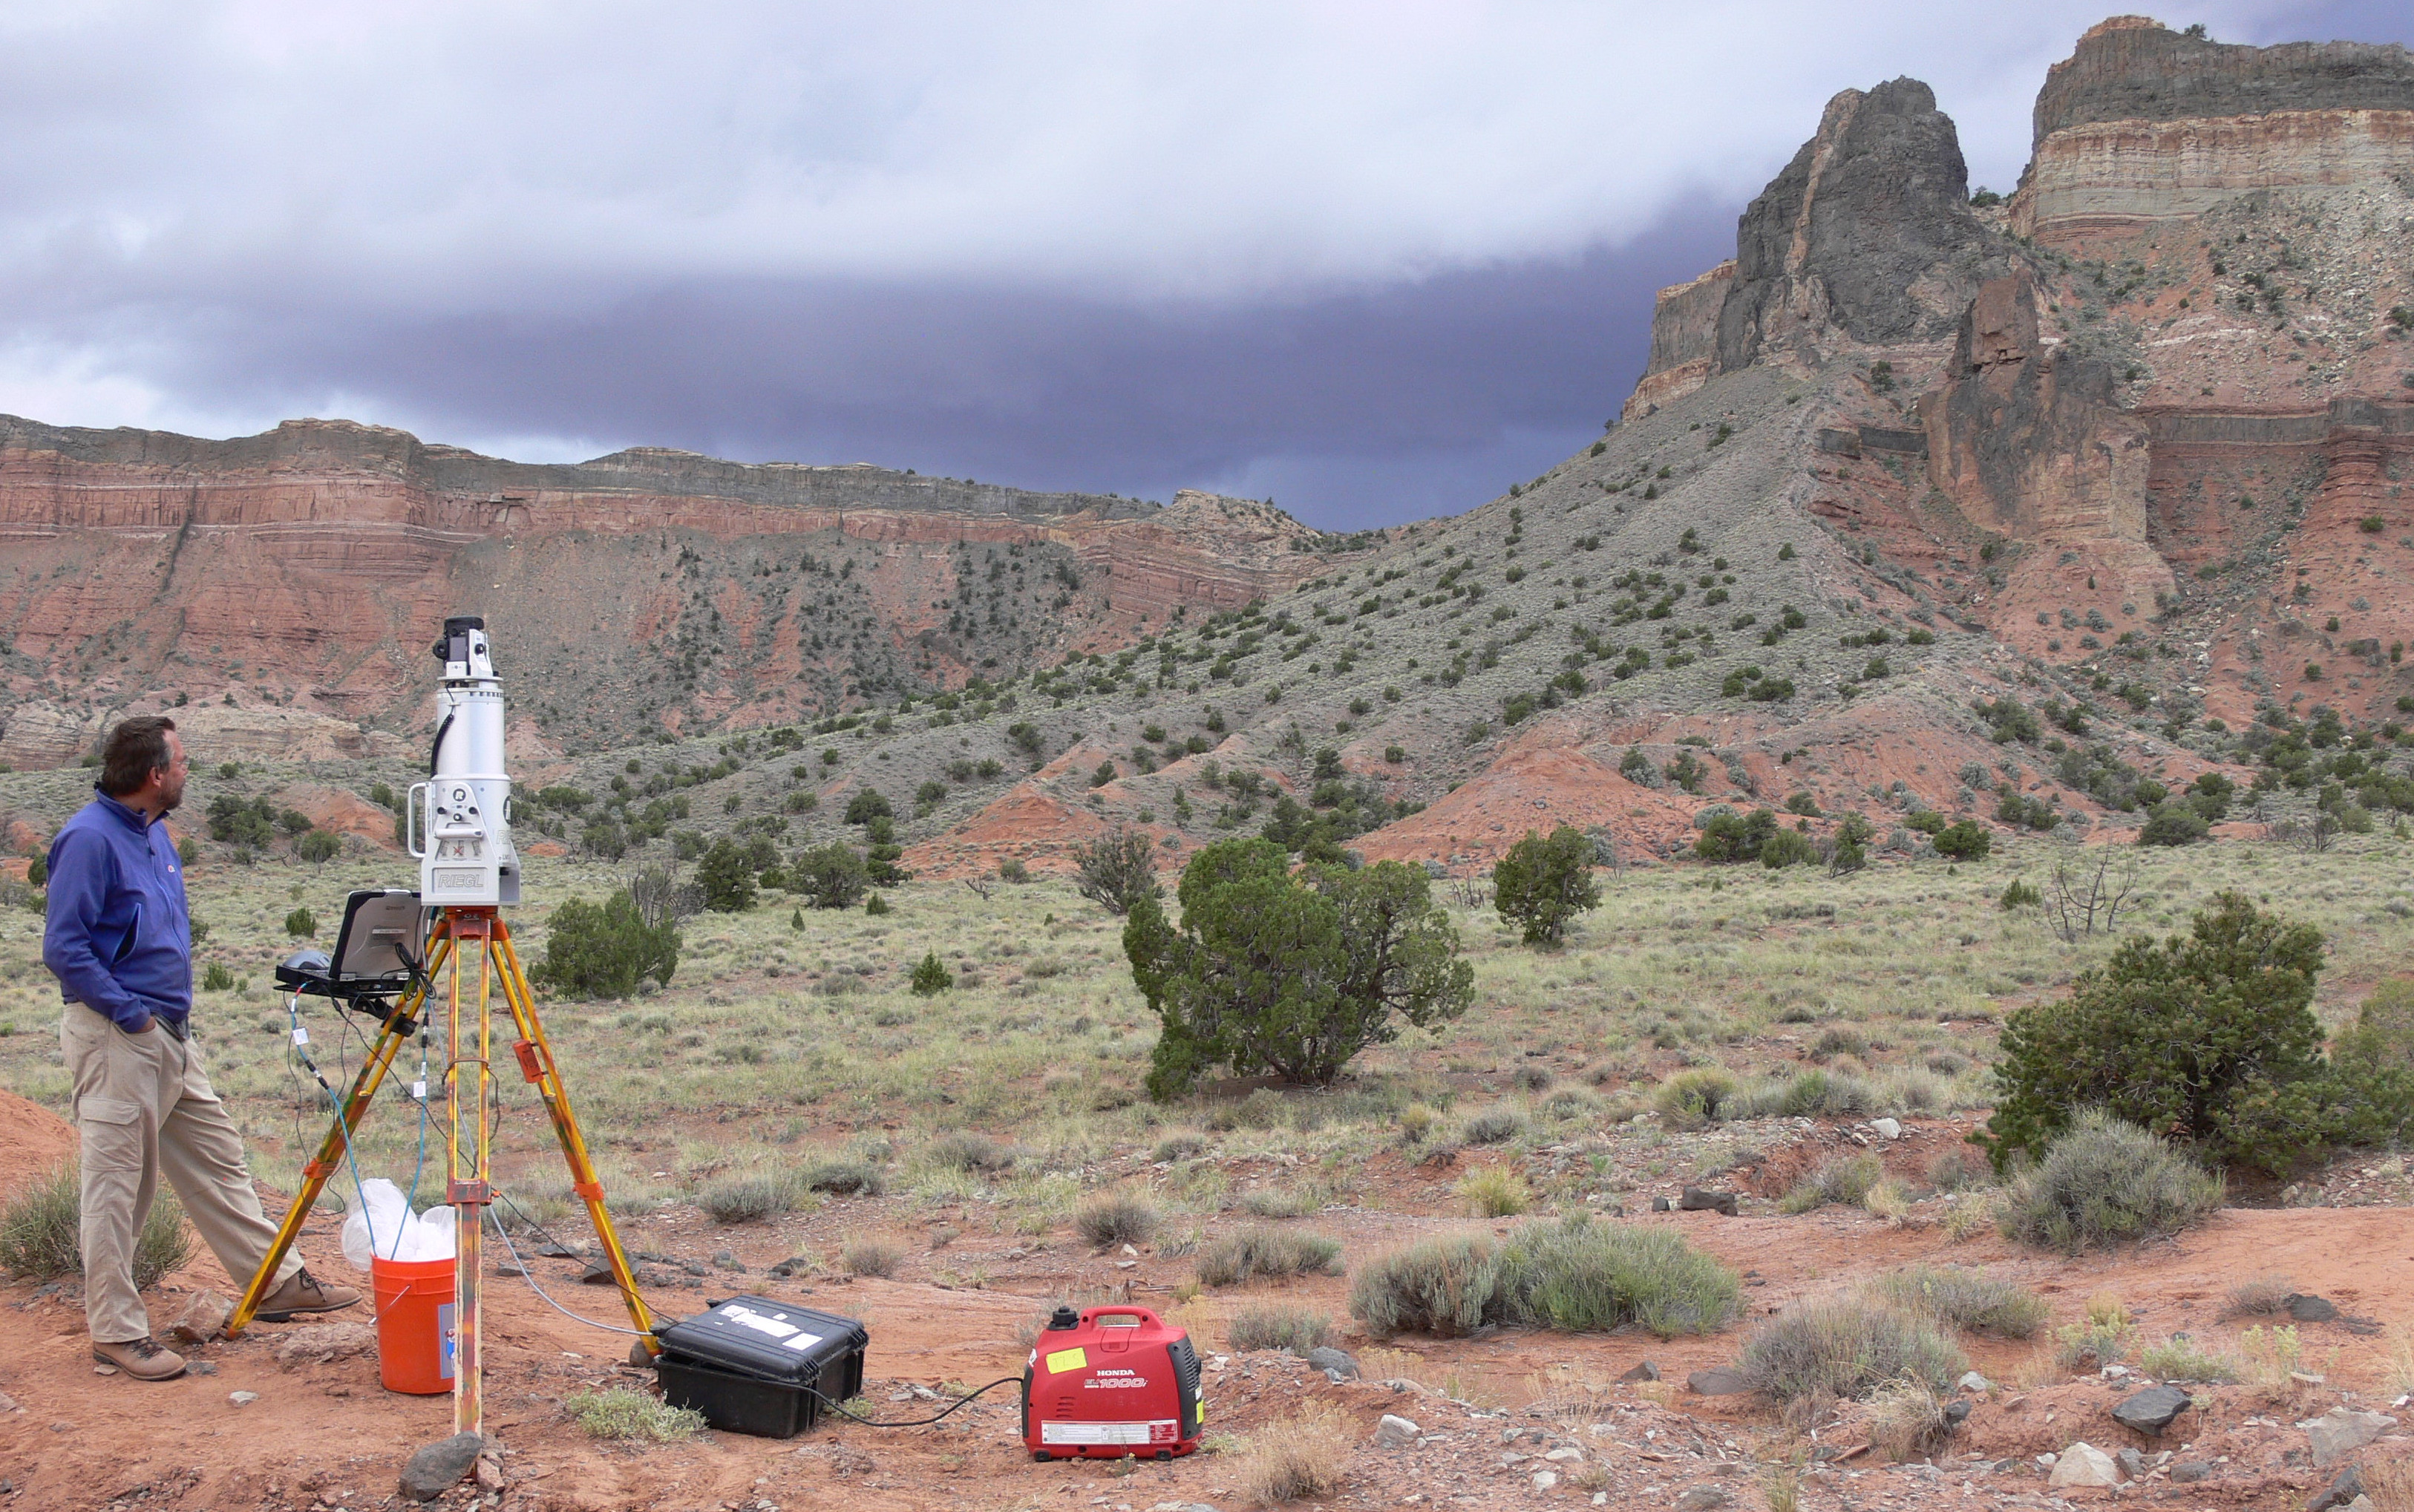
\includegraphics[width=1\textwidth]{figures/defense/ChuckConnor_Zlidar.jpg}
		\end{block}
	\column{.6\textwidth}
		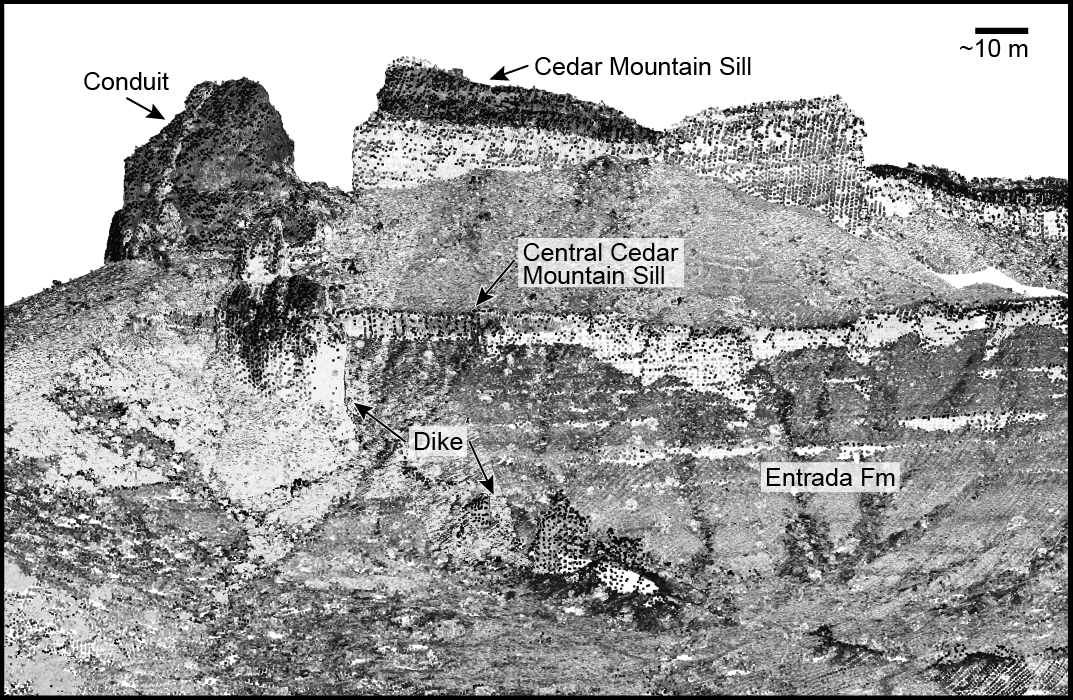
\includegraphics[width=1\textwidth]{figures/defense/CedarMtn-pcloud.png} 
	\end{columns}
		
	}

	\frame{\frametitle{Sills in the San Rafael Swell}
		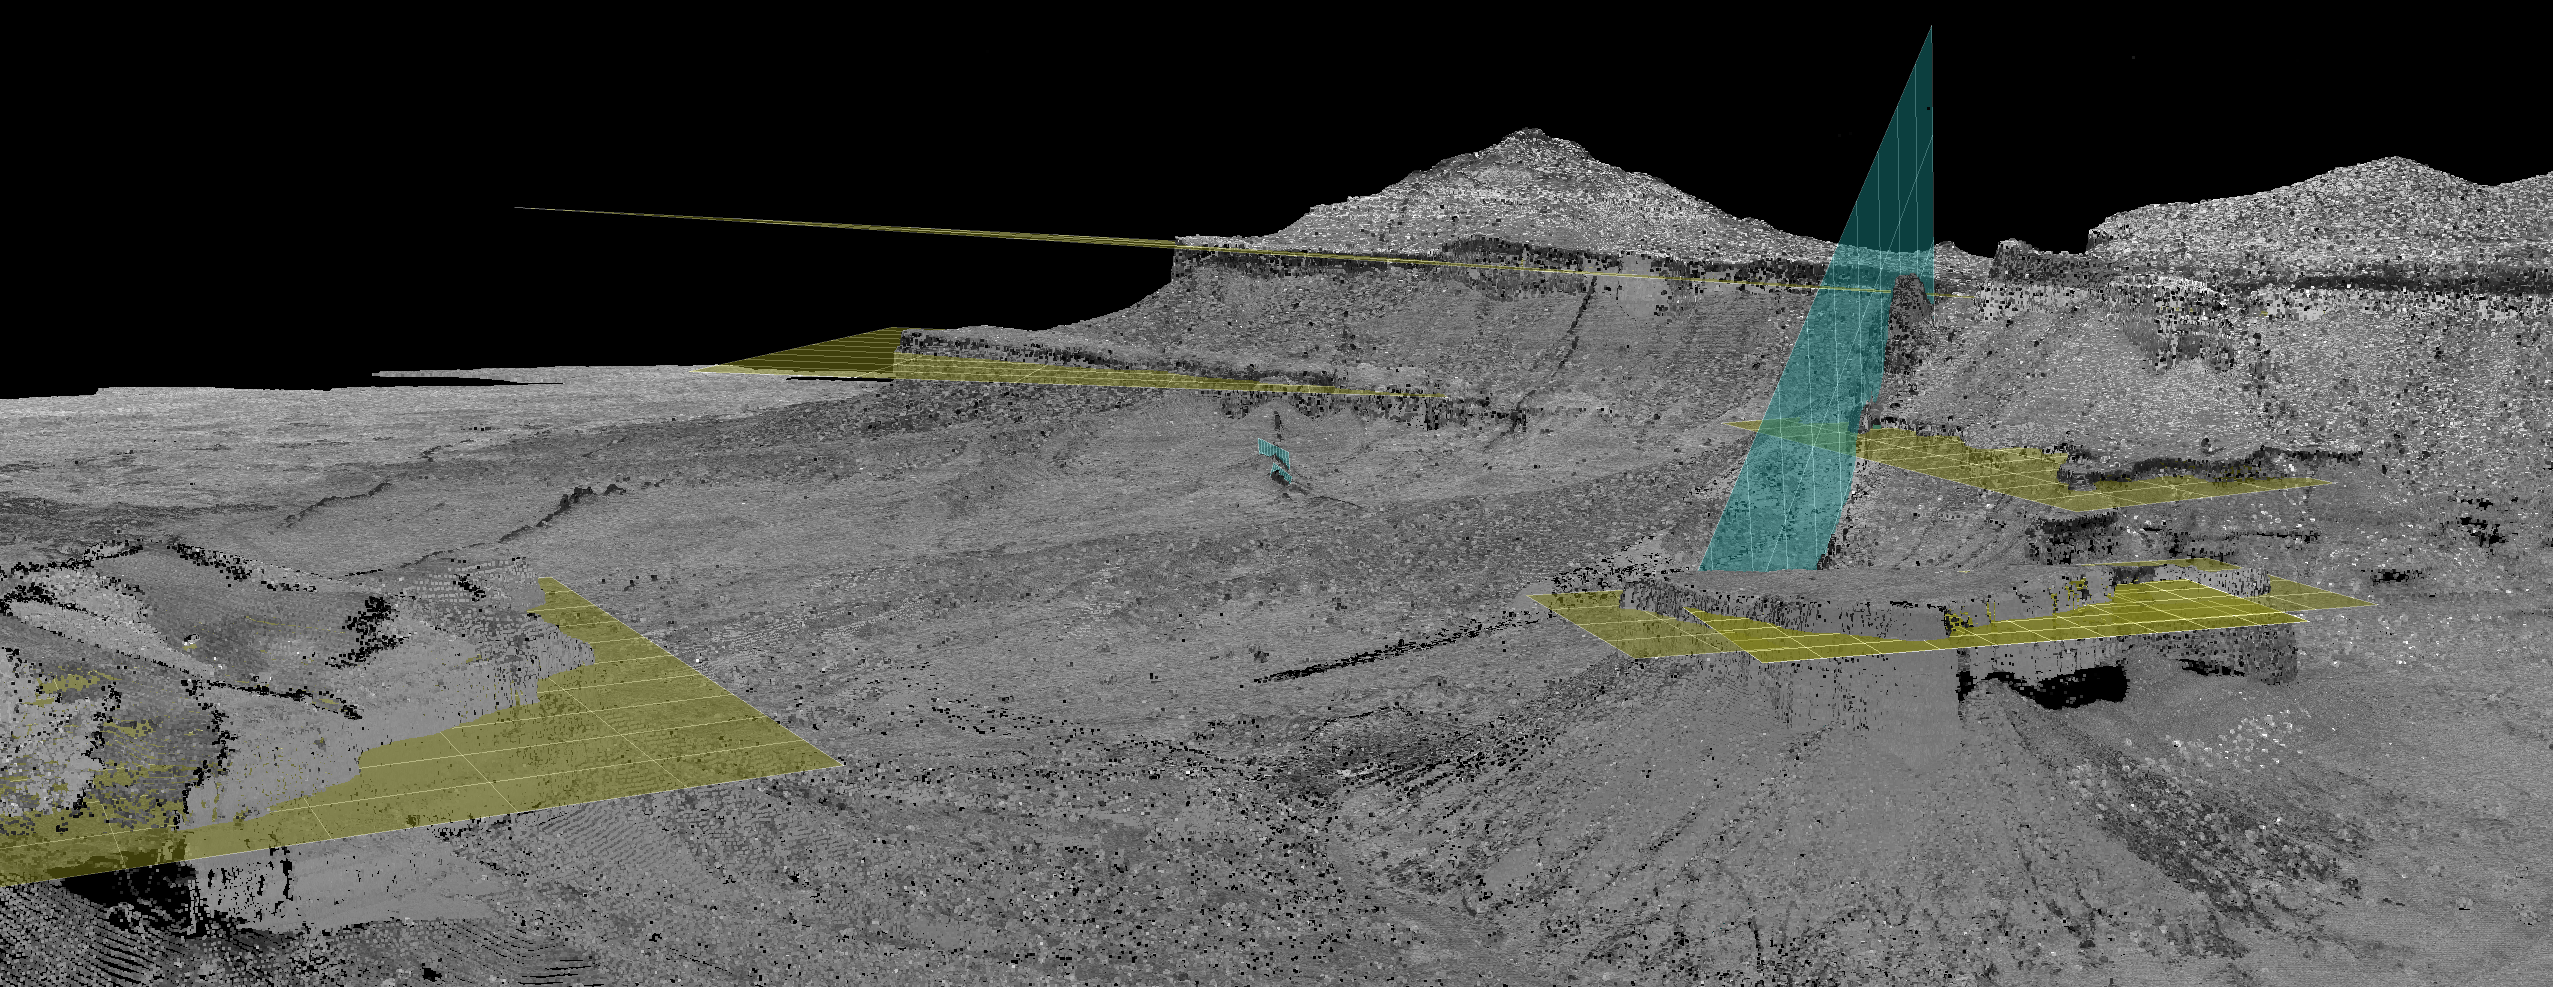
\includegraphics[width=1\textwidth]{figures/defense/lidar_screenshot.png}
	}

	\frame{\frametitle{Sills in the San Rafael Swell}
	\begin{columns}
	\column{.6\textwidth}
		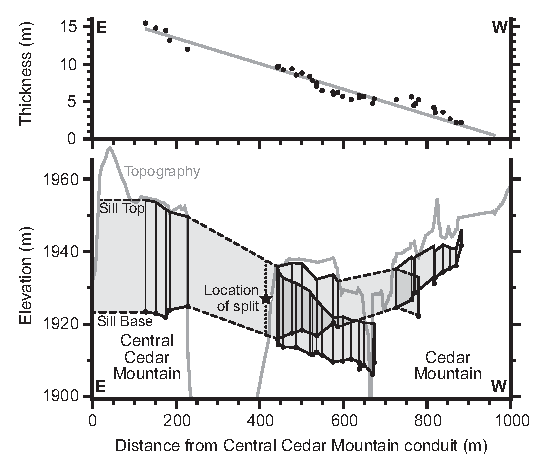
\includegraphics[width=0.5\textwidth]{figures/chapter-sills/Fig4-chart.eps}
		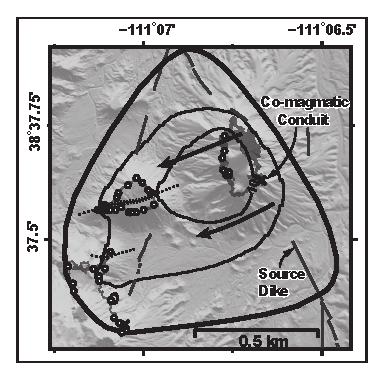
\includegraphics[width=0.5\textwidth]{figures/defense/ccm_model.eps}
	\column{.4\textwidth}
		\begin{block}{}
		\begin{itemize}
			\item Lidar
			\item Sills
			\item Total volume, geometry
			\item Modulation of eruption style
		\end{itemize}
		\end{block}
	\end{columns}
	}
	
%%%%%%%%%%%%%%%%%%%%%%%%%%%%%
%LAVA FLOWS
\subsection{Lava Flows}
	\frame{\frametitle{Lava Flows/Simulators}
		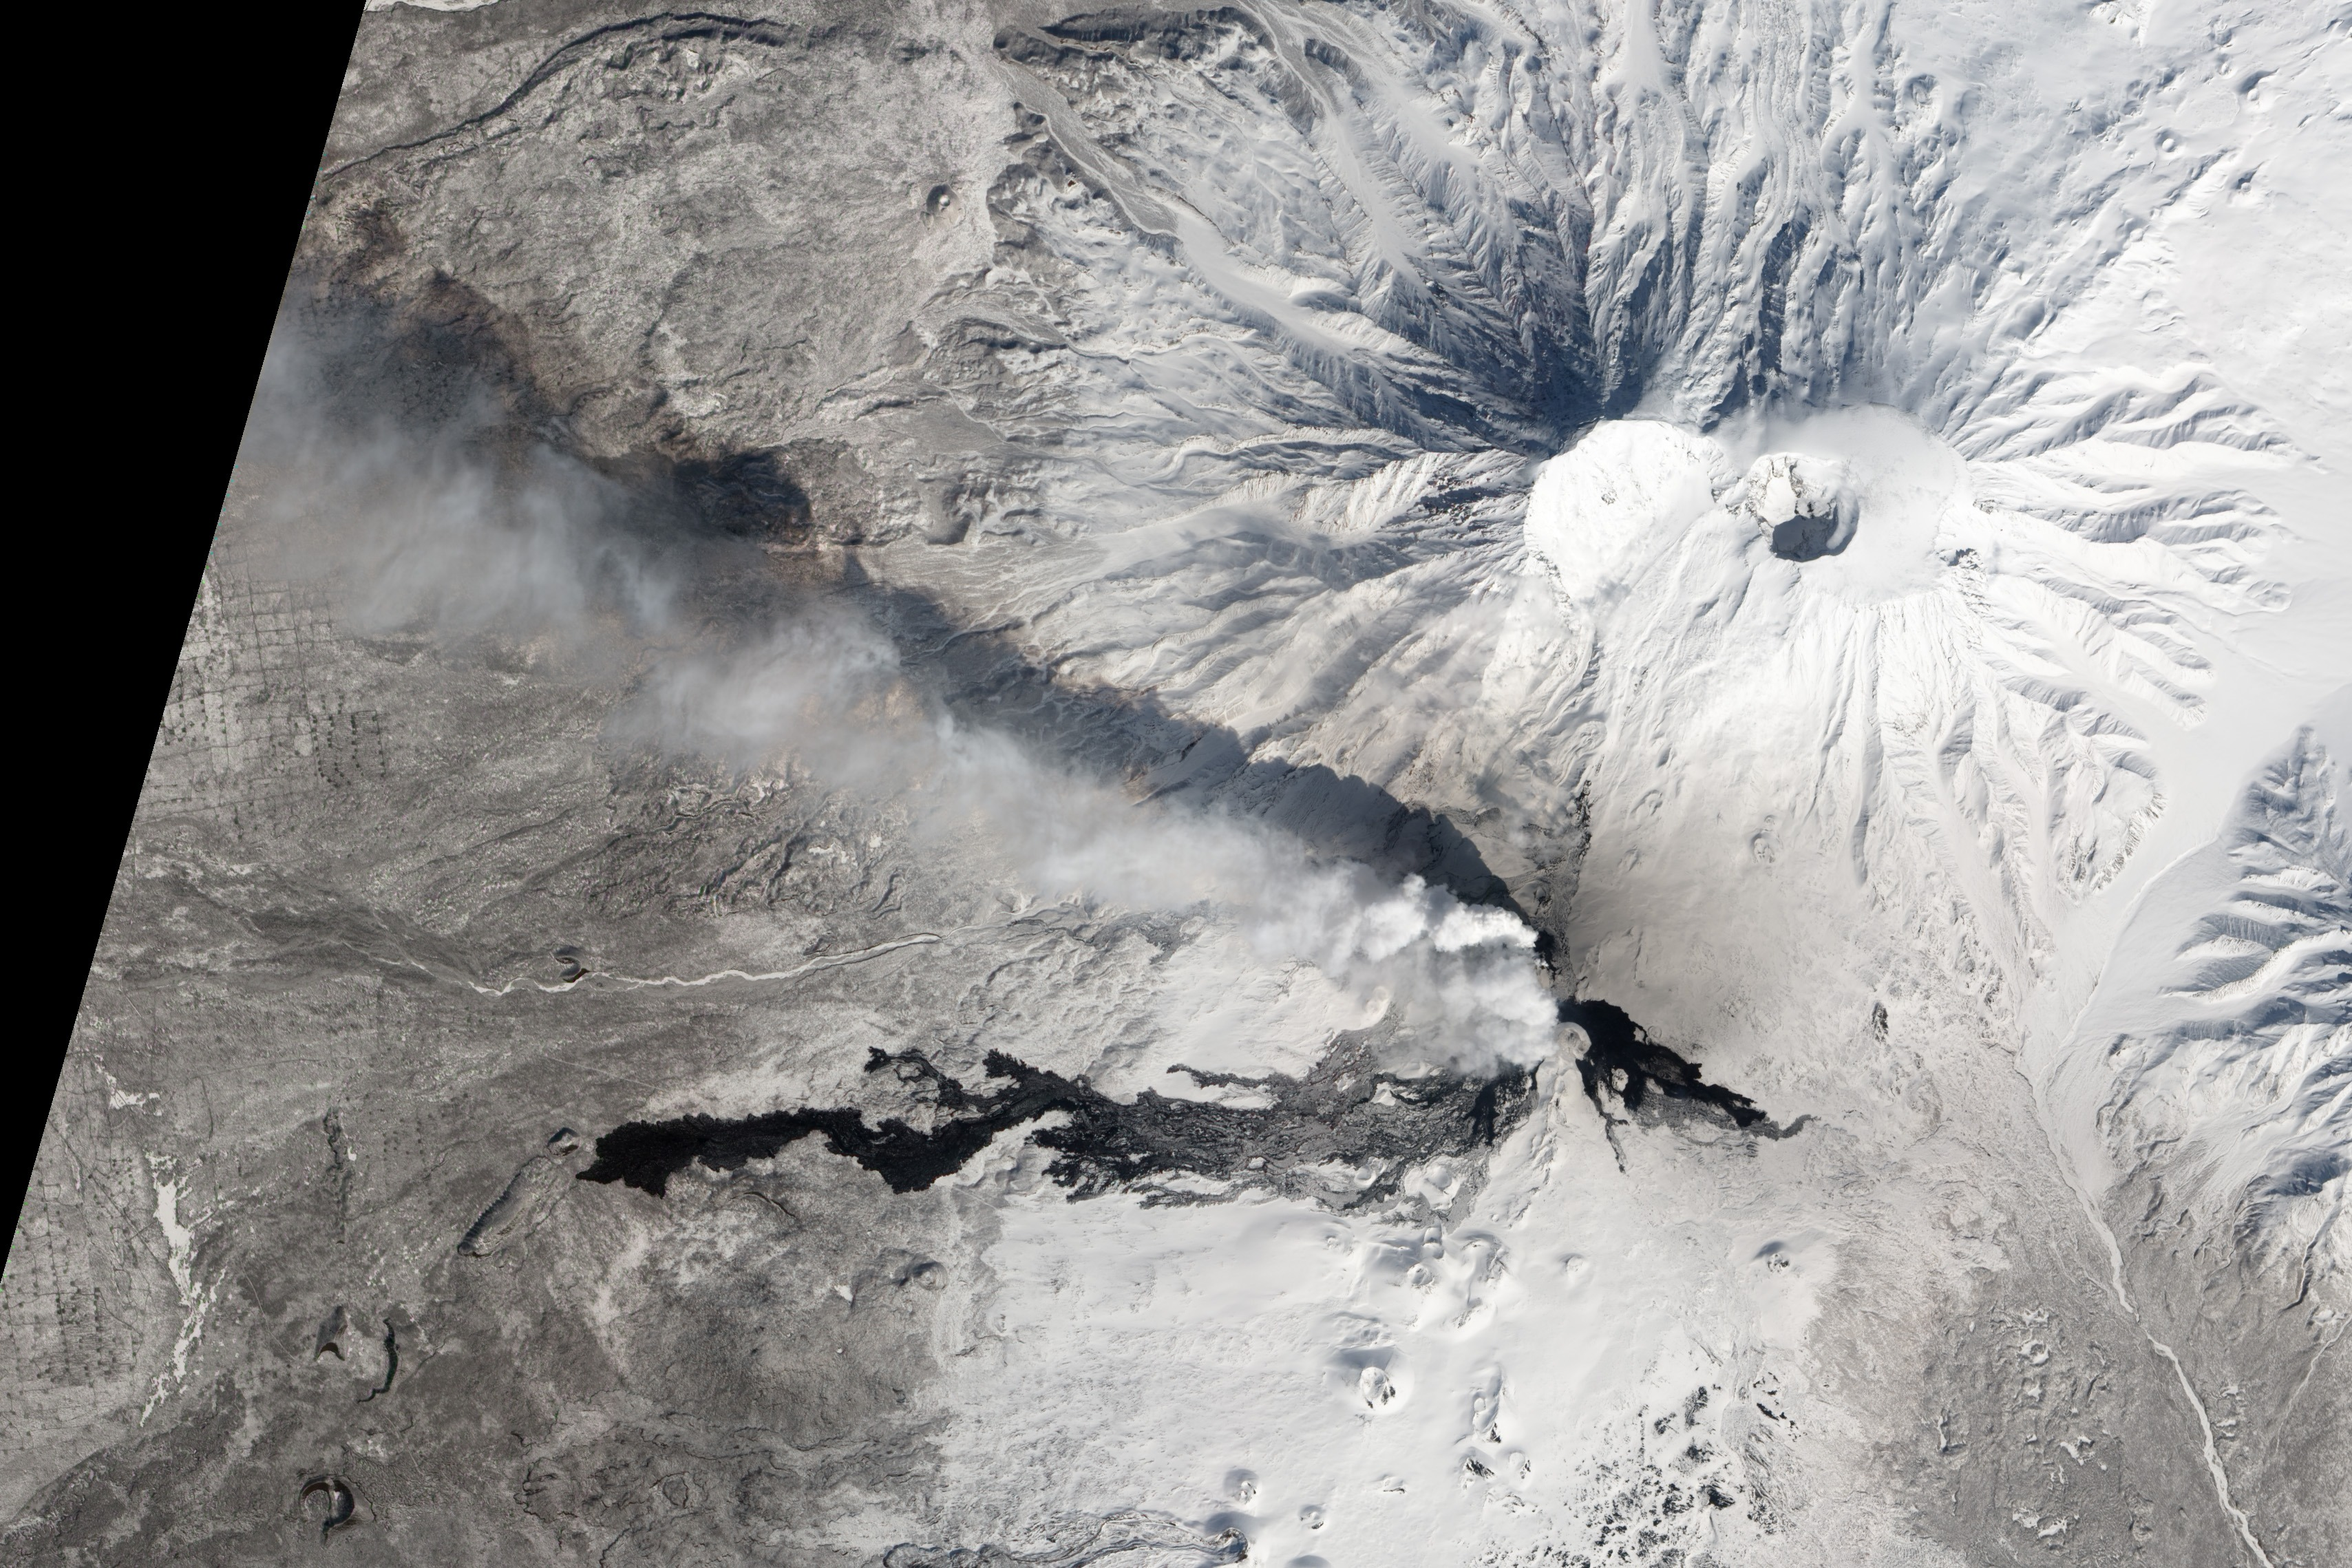
\includegraphics[width=1\textwidth,clip,trim=5cm 10cm 5cm 16cm]{figures/defense/tolbachik_eo1.png}
	}
	
	\frame{\frametitle{Lava Flows/Simulators}
	\begin{columns}
	\column{.23\textwidth}
		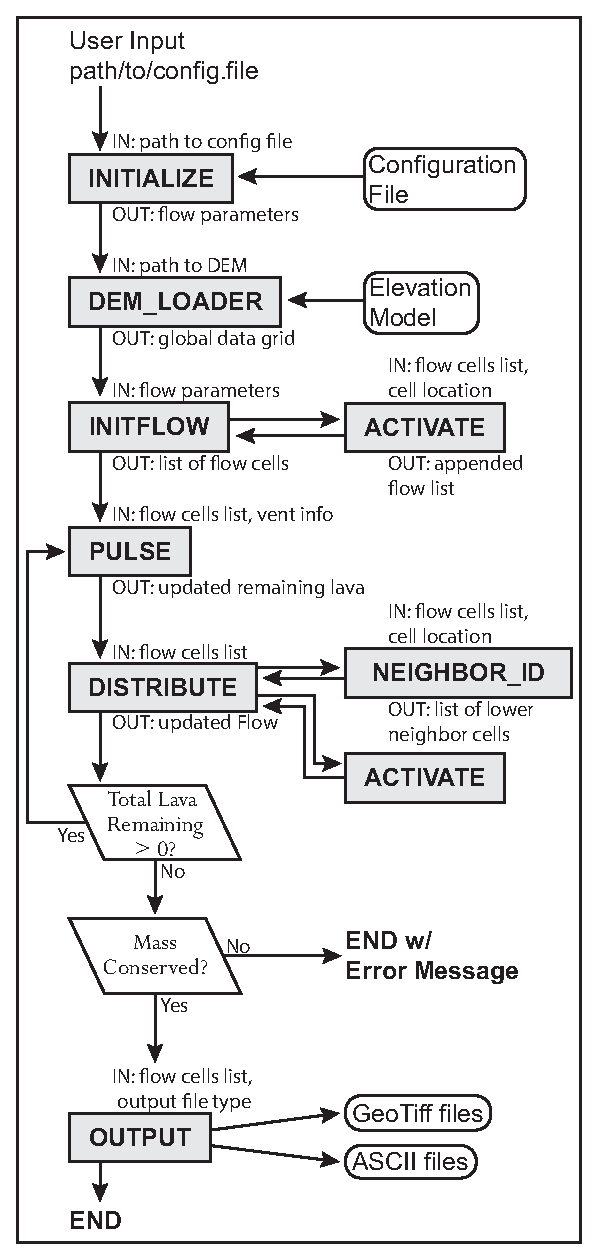
\includegraphics[width=1\textwidth]{figures/chapter-molasses/Flow_Chart.eps}
	\column{.77\textwidth}
		\begin{block}{MOLASSES --- Modular Lava Simulation Software}
		\begin{columns}
		\column{.5\textwidth}
			\begin{itemize}
				\item MOLASSES
				\item CA Code
			\end{itemize}
		\column{.5\textwidth}
			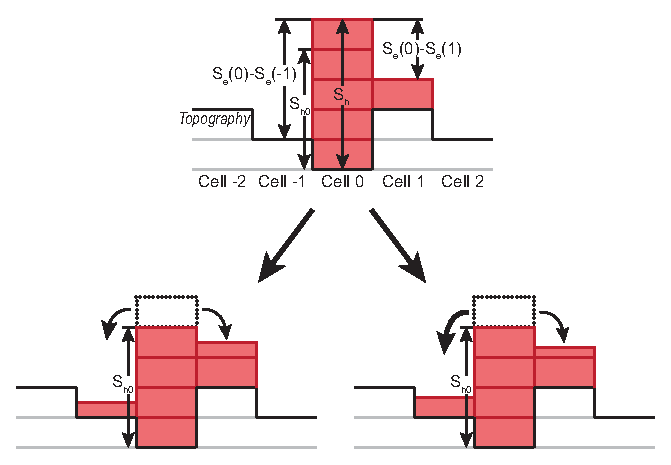
\includegraphics[width=1\textwidth]{figures/chapter-molasses/slope-proportional-example.eps}
		\end{columns}
		\end{block}
	\end{columns}
	}

	\frame{\frametitle{Lava Flows/Simulators}
	\begin{columns}
	\column{.5\textwidth}
		\begin{block}{}
		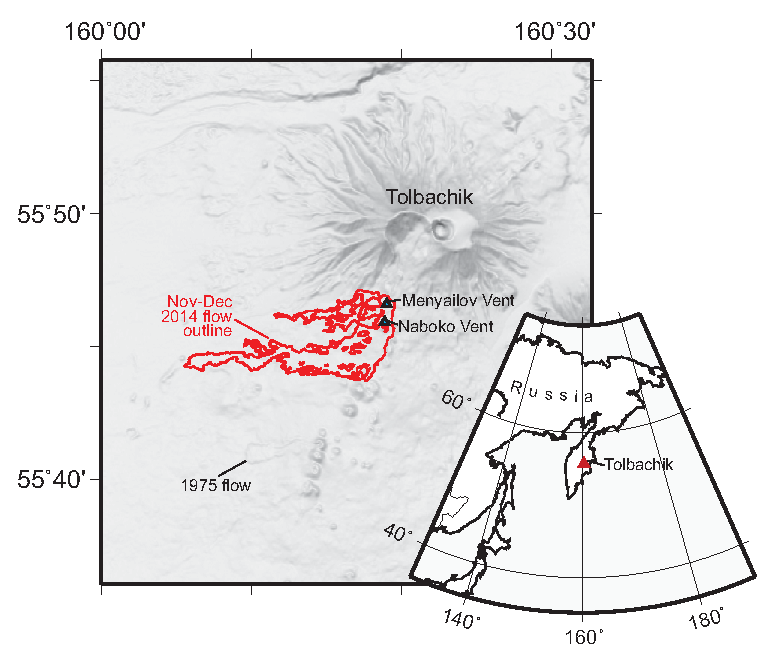
\includegraphics[width=1\textwidth]{figures/chapter-molasses/locator_complete.eps}
		\end{block}
	\column{.5\textwidth}
		\begin{block}{}
		Validation
		\includegraphics[width=1\textwidth]{figures/defense/pulse_examples.eps}
		\end{block}
	\end{columns}
	}


%%%%%%%%%%%%%%%%%%%%%%%%%%%%%
%Vent Density
\subsection{Vent Density}
	\frame{\frametitle{Spatial Density of Clusters}
		\begin{block}{}
		\end{block}
		\begin{block}{}
			\begin{columns}
			\column{.4\textwidth}
				\centering
				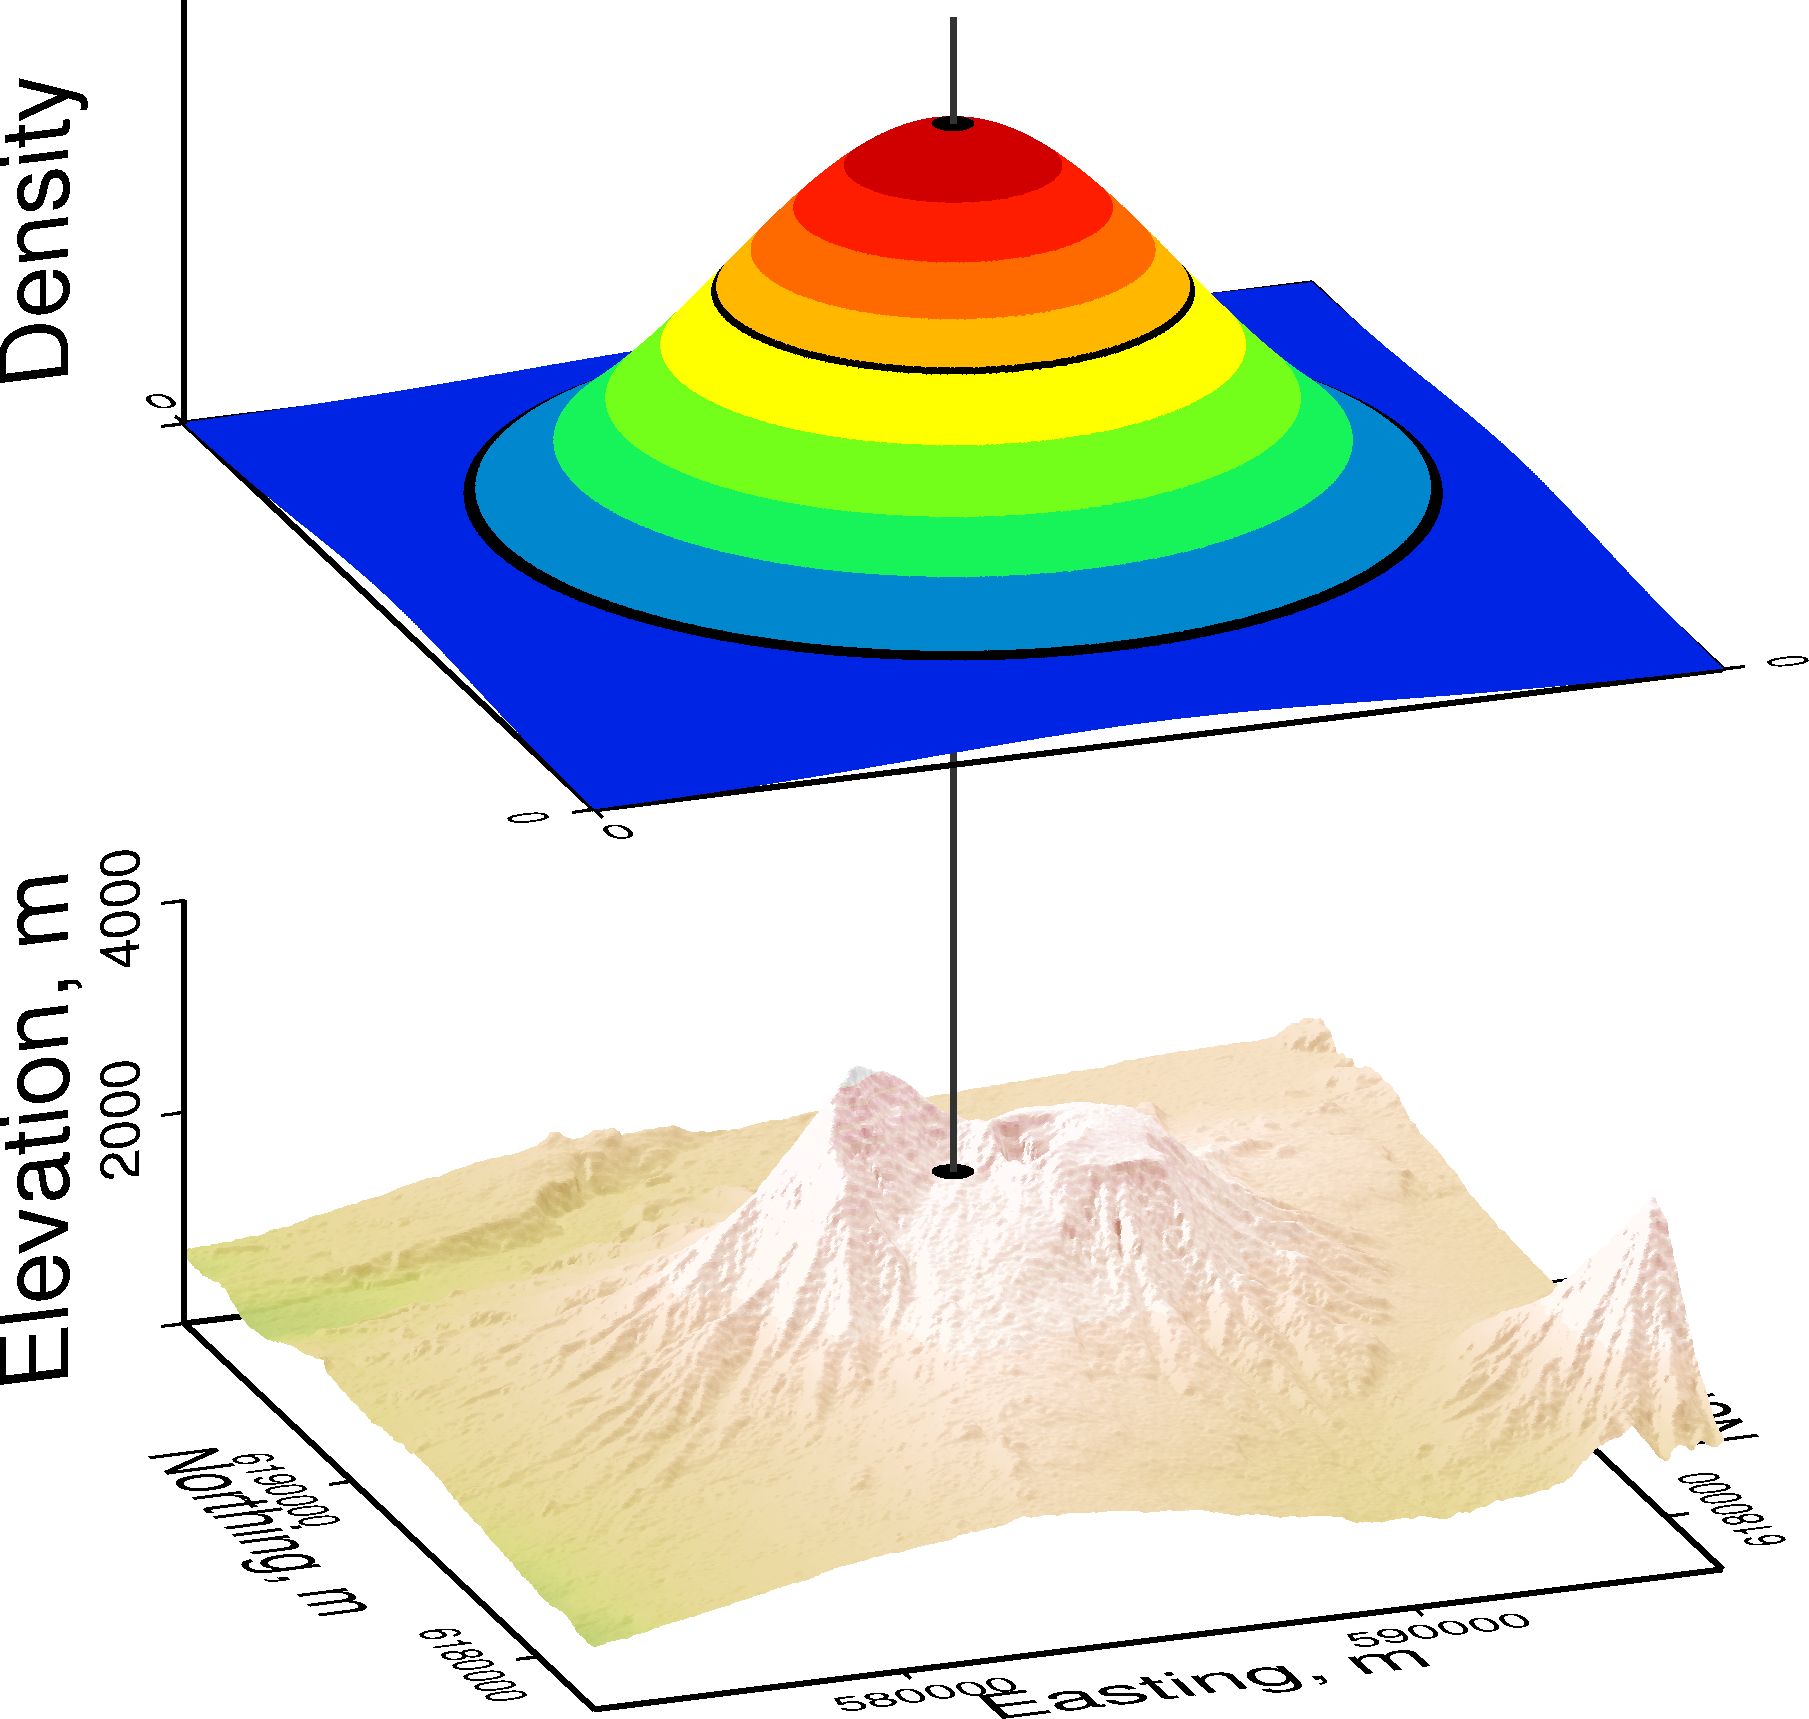
\includegraphics[width=0.8\textwidth]{figures/defense/volcano-density.png}
			\column{.6\textwidth}
				\centering
				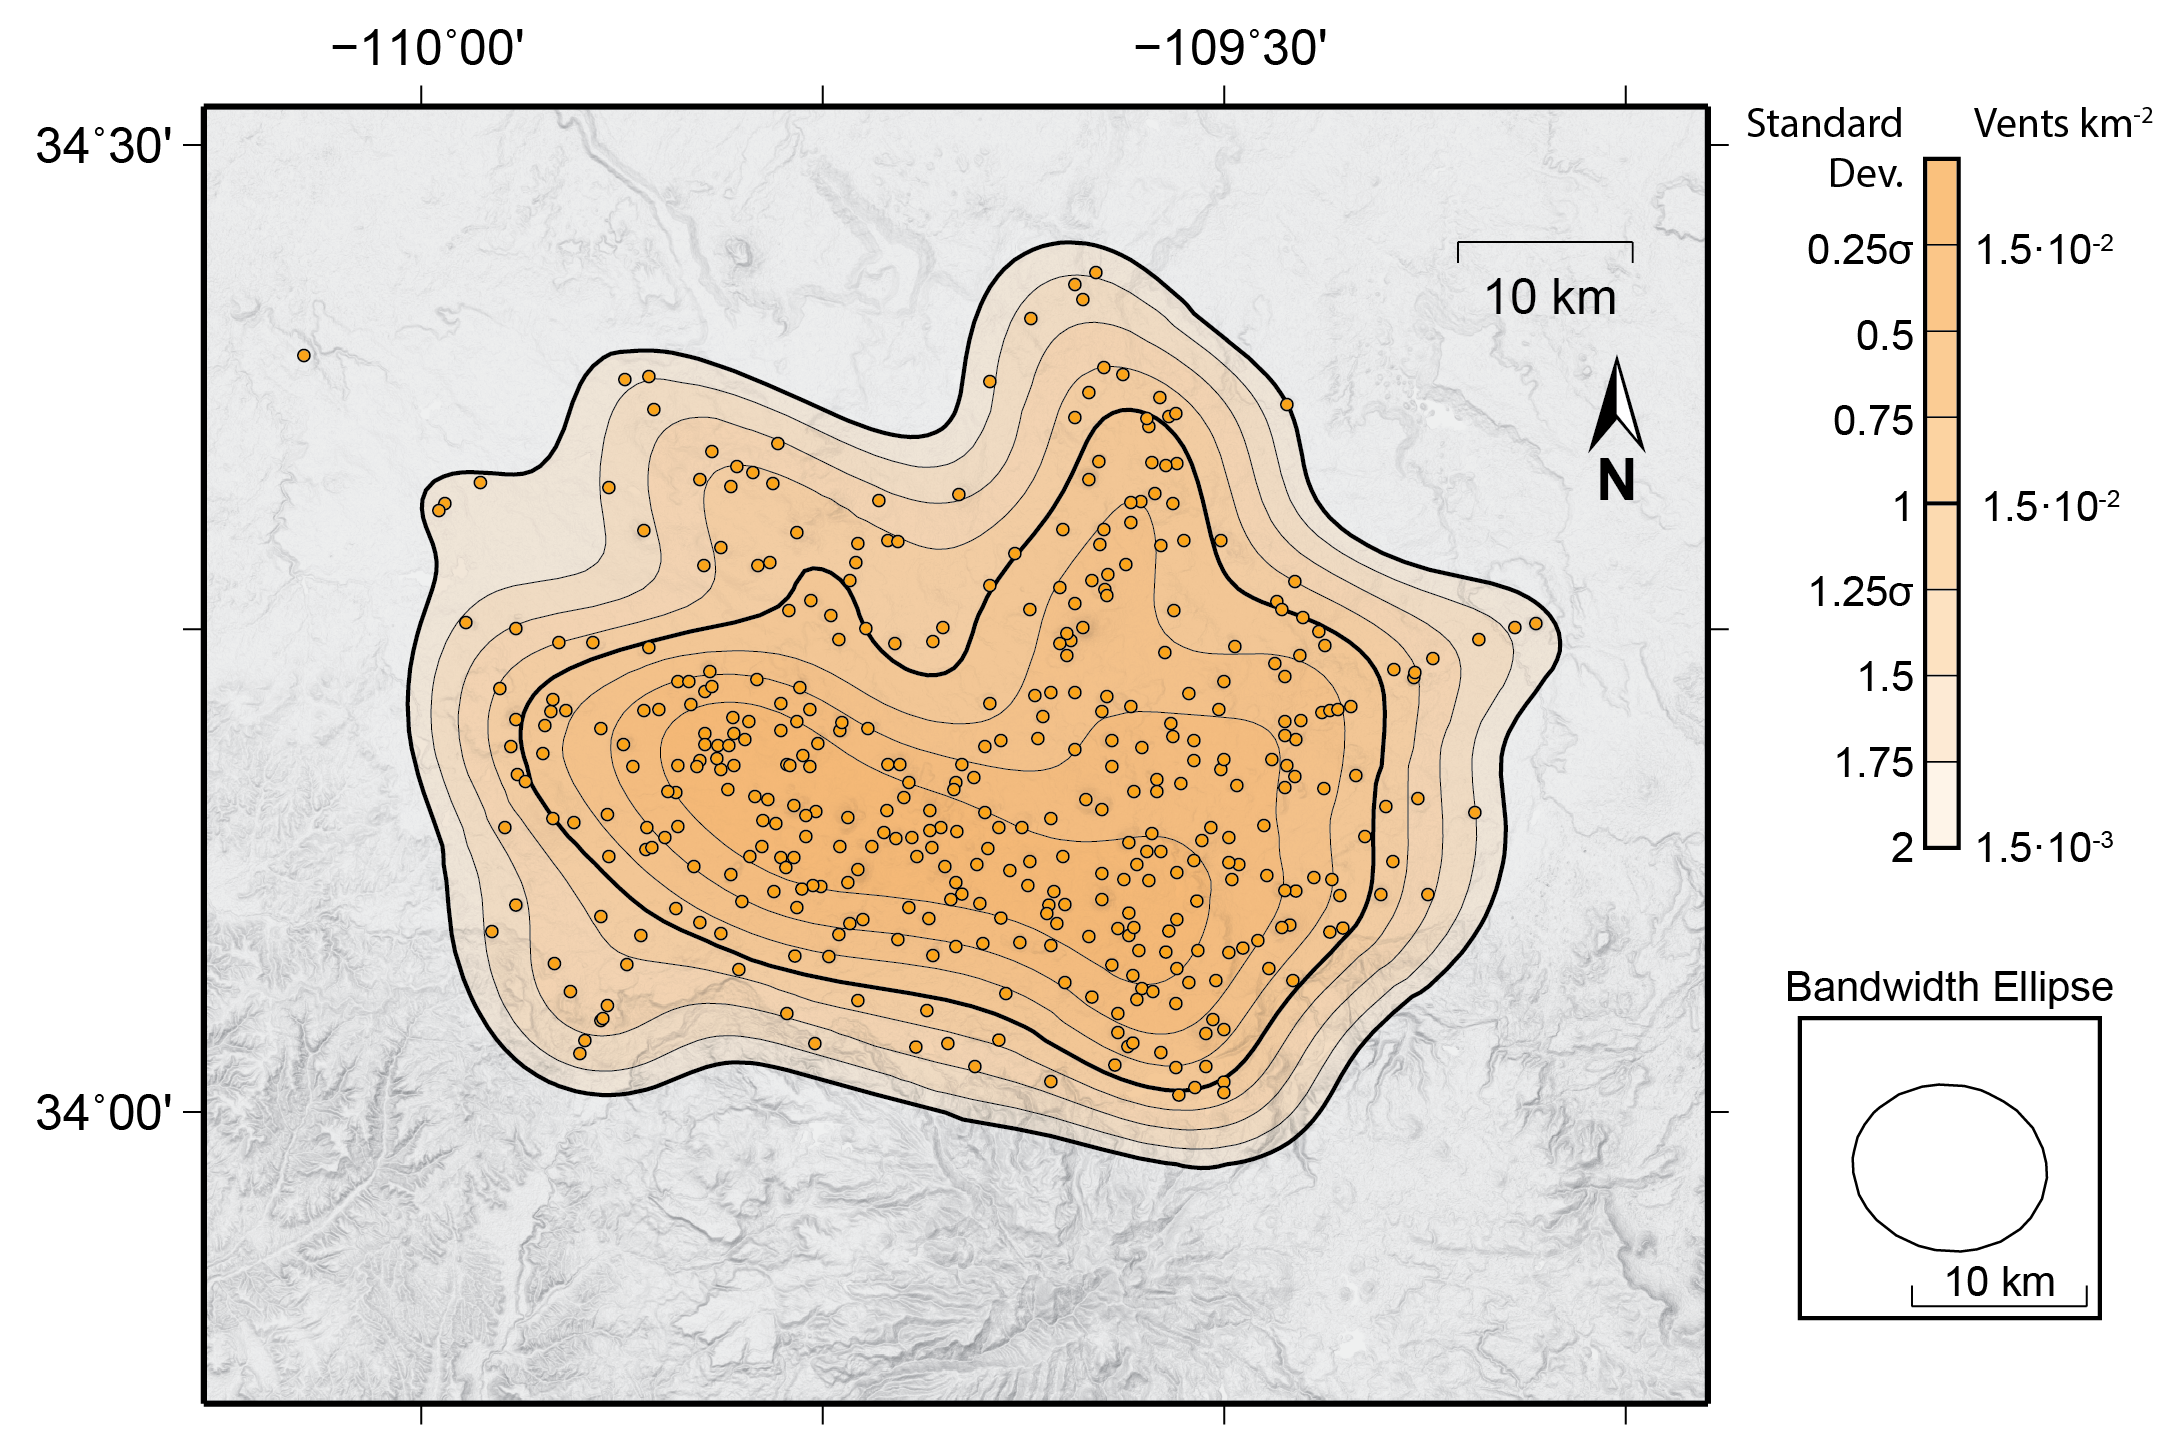
\includegraphics[width=0.8\textwidth]{figures/chapter-spatial_density/springerville_kde_300dpi.png}
			\end{columns}
		\end{block}
	}

	\frame{\frametitle{Spatial Density of Clusters}
		\begin{columns}
		\column{.2\textwidth}
			\begin{centering}
			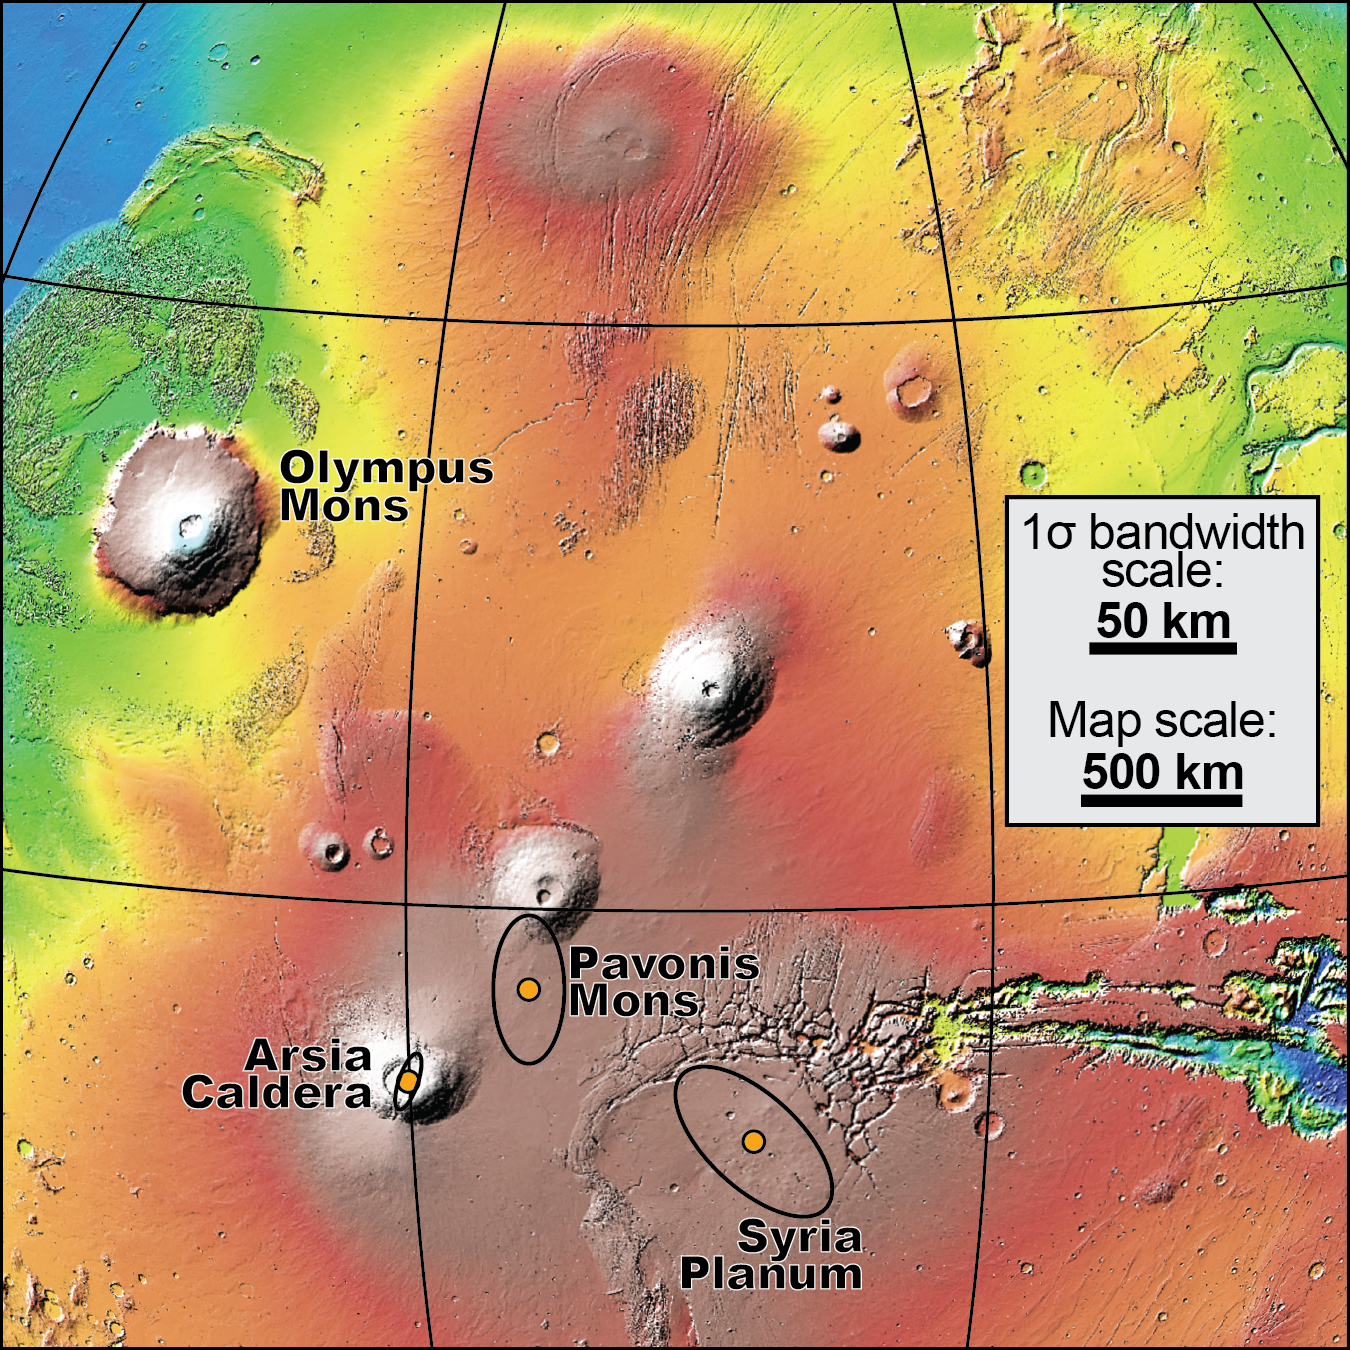
\includegraphics[width=0.8\textwidth]{figures/defense/mars_locator_300dpi}
			
			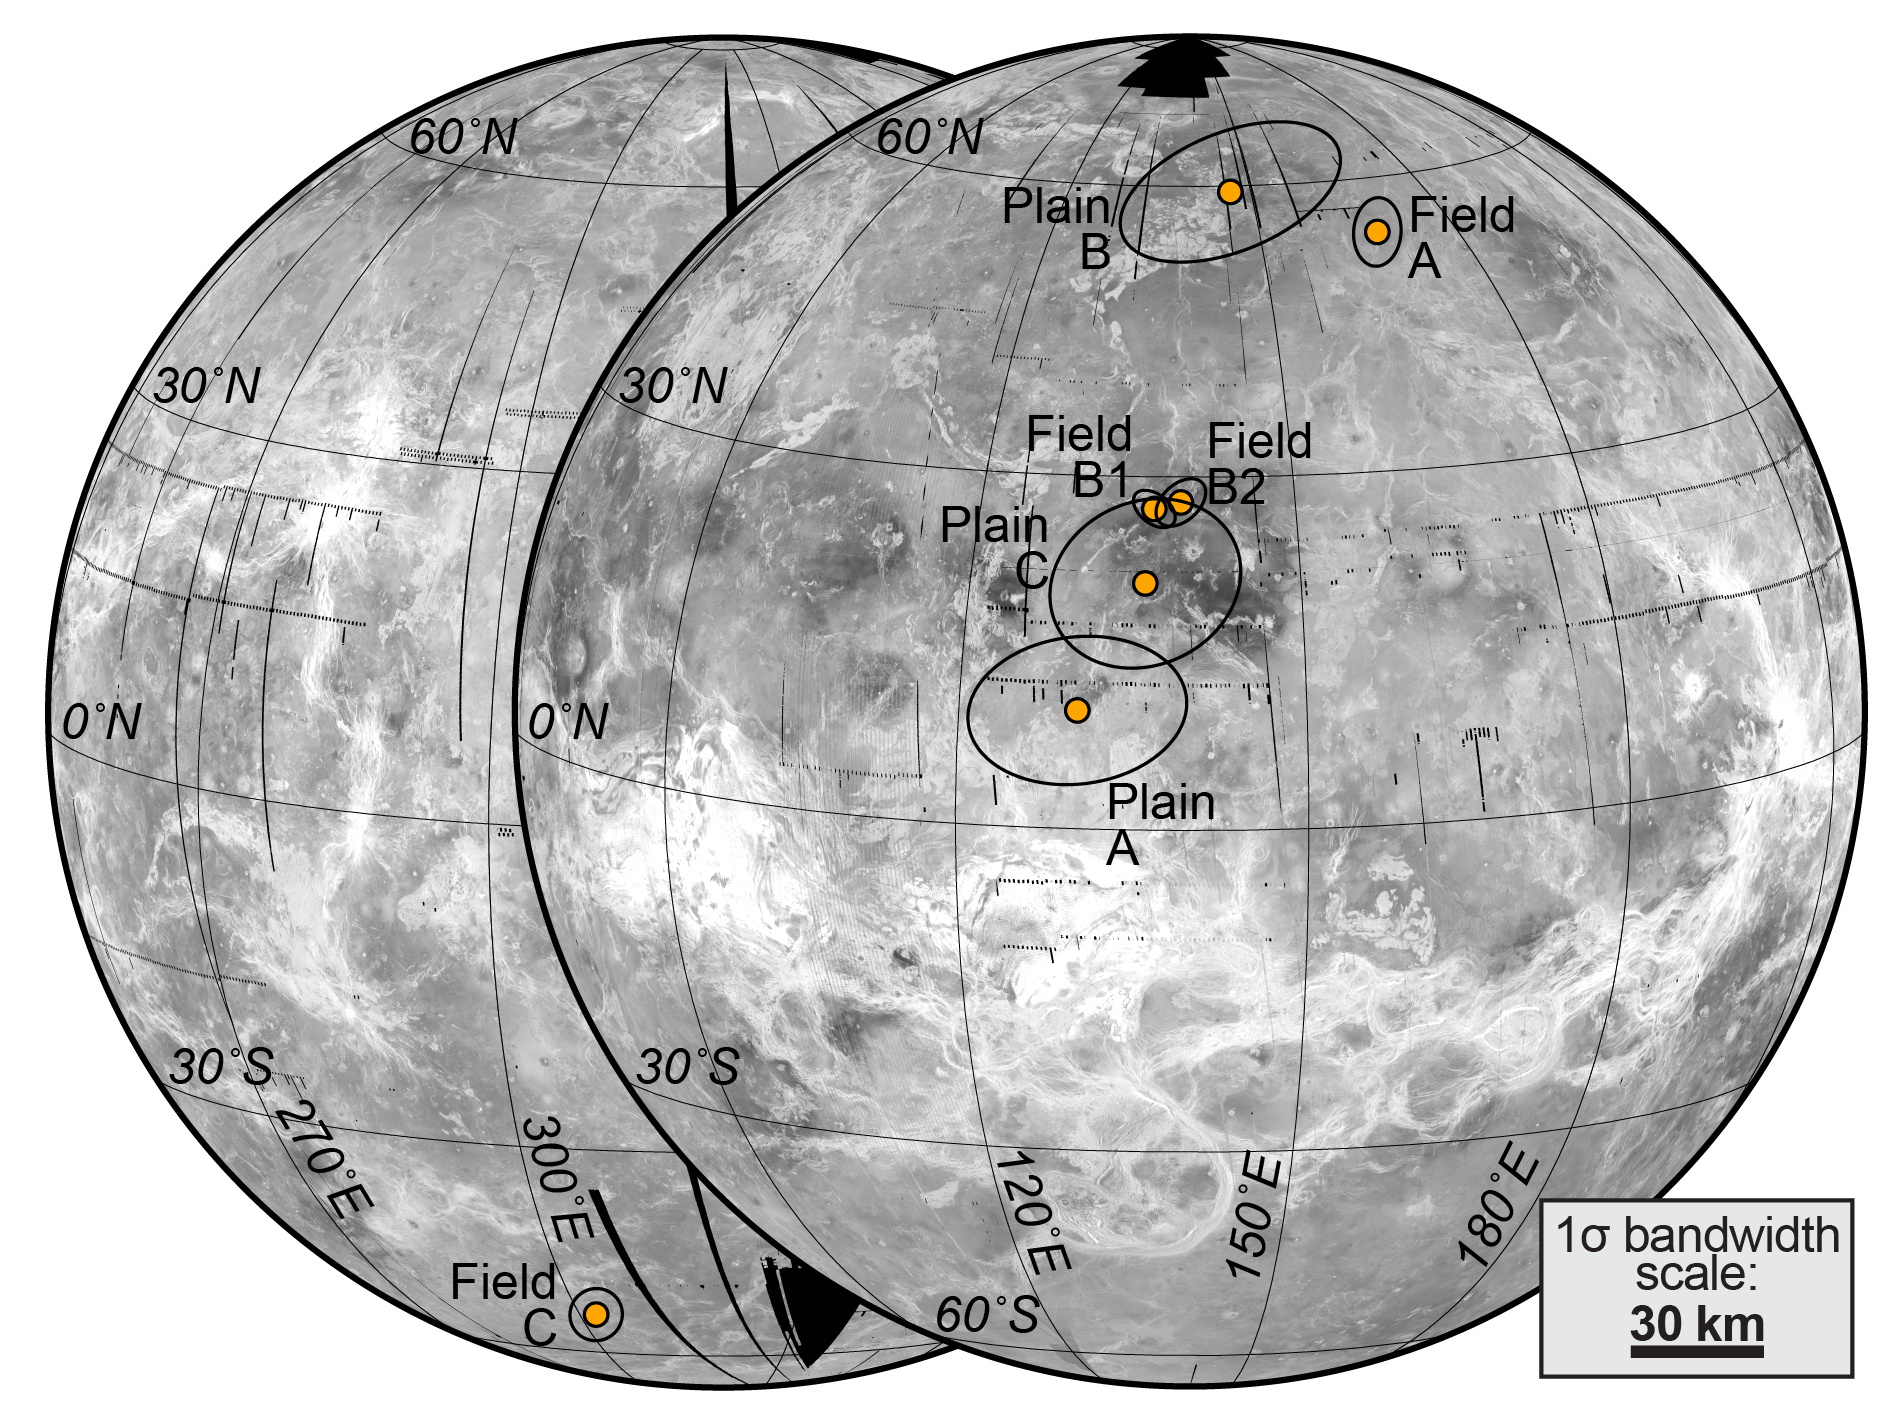
\includegraphics[width=1\textwidth]{figures/defense/venus_globe_300dpi}
			
			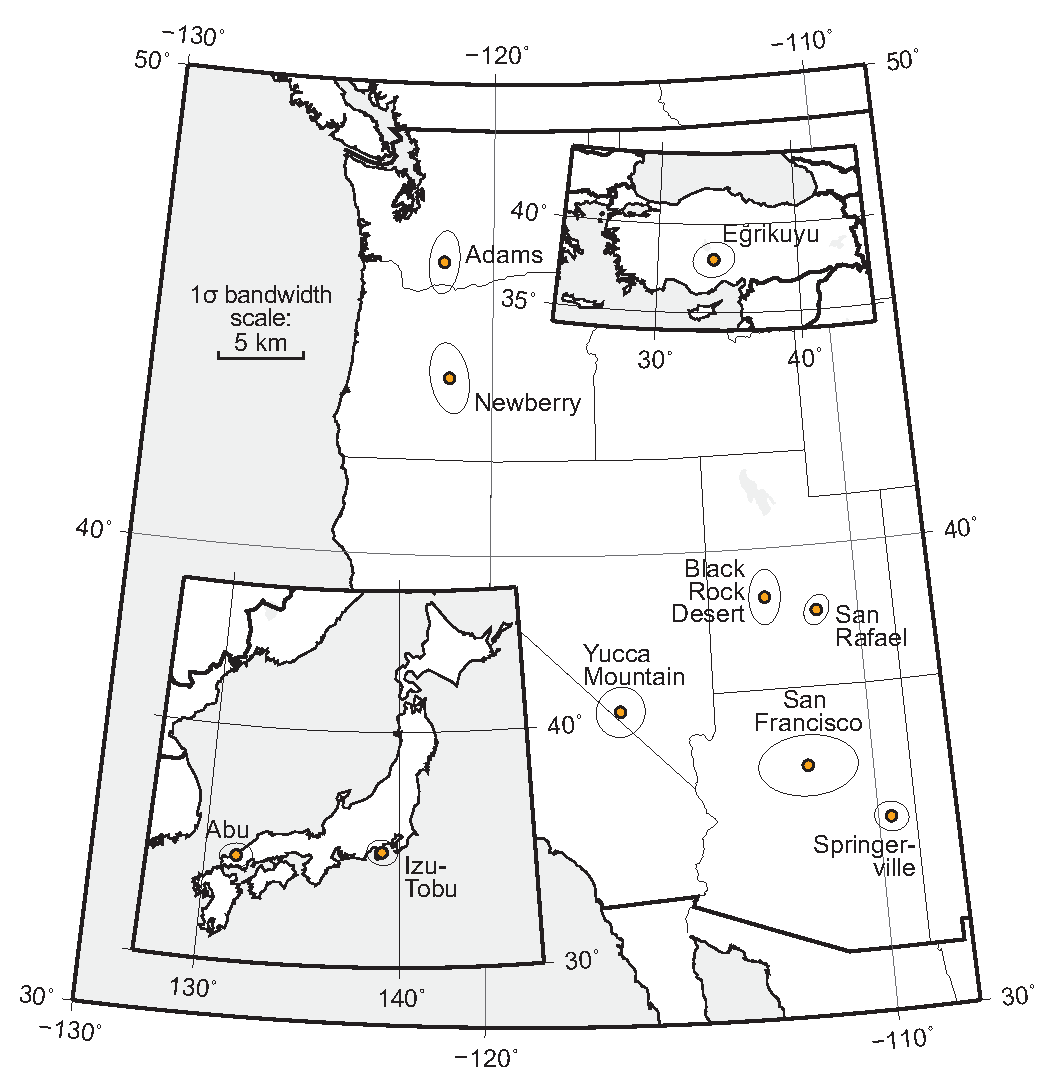
\includegraphics[width=0.9\textwidth]{figures/chapter-spatial_density/locators/earth_locator.eps}
			\end{centering}
		\column{.7\textwidth}
			\begin{block}{Average Vent Intensity}
			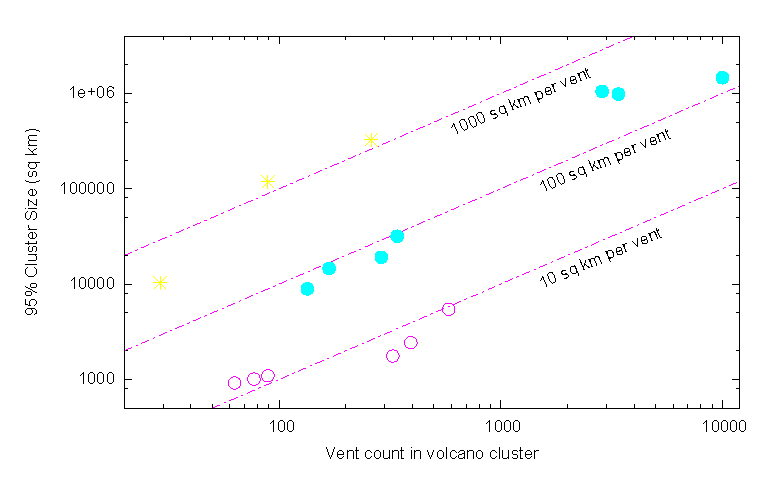
\includegraphics[width=0.9\textwidth]{figures/defense/cluster_dens.eps}
			\end{block}
			%% GNUPLOT: LaTeX picture
\setlength{\unitlength}{0.240900pt}
\ifx\plotpoint\undefined\newsavebox{\plotpoint}\fi
\sbox{\plotpoint}{\rule[-0.200pt]{0.400pt}{0.400pt}}%
\begin{picture}(1500,900)(0,0)
\sbox{\plotpoint}{\rule[-0.200pt]{0.400pt}{0.400pt}}%
\put(231.0,131.0){\rule[-0.200pt]{2.409pt}{0.400pt}}
\put(1429.0,131.0){\rule[-0.200pt]{2.409pt}{0.400pt}}
\put(231.0,169.0){\rule[-0.200pt]{2.409pt}{0.400pt}}
\put(1429.0,169.0){\rule[-0.200pt]{2.409pt}{0.400pt}}
\put(231.0,187.0){\rule[-0.200pt]{4.818pt}{0.400pt}}
\put(211,187){\makebox(0,0)[r]{ 1000}}
\put(1419.0,187.0){\rule[-0.200pt]{4.818pt}{0.400pt}}
\put(231.0,243.0){\rule[-0.200pt]{2.409pt}{0.400pt}}
\put(1429.0,243.0){\rule[-0.200pt]{2.409pt}{0.400pt}}
\put(231.0,318.0){\rule[-0.200pt]{2.409pt}{0.400pt}}
\put(1429.0,318.0){\rule[-0.200pt]{2.409pt}{0.400pt}}
\put(231.0,356.0){\rule[-0.200pt]{2.409pt}{0.400pt}}
\put(1429.0,356.0){\rule[-0.200pt]{2.409pt}{0.400pt}}
\put(231.0,374.0){\rule[-0.200pt]{4.818pt}{0.400pt}}
\put(211,374){\makebox(0,0)[r]{ 10000}}
\put(1419.0,374.0){\rule[-0.200pt]{4.818pt}{0.400pt}}
\put(231.0,430.0){\rule[-0.200pt]{2.409pt}{0.400pt}}
\put(1429.0,430.0){\rule[-0.200pt]{2.409pt}{0.400pt}}
\put(231.0,504.0){\rule[-0.200pt]{2.409pt}{0.400pt}}
\put(1429.0,504.0){\rule[-0.200pt]{2.409pt}{0.400pt}}
\put(231.0,542.0){\rule[-0.200pt]{2.409pt}{0.400pt}}
\put(1429.0,542.0){\rule[-0.200pt]{2.409pt}{0.400pt}}
\put(231.0,560.0){\rule[-0.200pt]{4.818pt}{0.400pt}}
\put(211,560){\makebox(0,0)[r]{ 100000}}
\put(1419.0,560.0){\rule[-0.200pt]{4.818pt}{0.400pt}}
\put(231.0,616.0){\rule[-0.200pt]{2.409pt}{0.400pt}}
\put(1429.0,616.0){\rule[-0.200pt]{2.409pt}{0.400pt}}
\put(231.0,691.0){\rule[-0.200pt]{2.409pt}{0.400pt}}
\put(1429.0,691.0){\rule[-0.200pt]{2.409pt}{0.400pt}}
\put(231.0,729.0){\rule[-0.200pt]{2.409pt}{0.400pt}}
\put(1429.0,729.0){\rule[-0.200pt]{2.409pt}{0.400pt}}
\put(231.0,747.0){\rule[-0.200pt]{4.818pt}{0.400pt}}
\put(211,747){\makebox(0,0)[r]{ 1e+06}}
\put(1419.0,747.0){\rule[-0.200pt]{4.818pt}{0.400pt}}
\put(231.0,803.0){\rule[-0.200pt]{2.409pt}{0.400pt}}
\put(1429.0,803.0){\rule[-0.200pt]{2.409pt}{0.400pt}}
\put(231.0,131.0){\rule[-0.200pt]{0.400pt}{2.409pt}}
\put(231.0,849.0){\rule[-0.200pt]{0.400pt}{2.409pt}}
\put(308.0,131.0){\rule[-0.200pt]{0.400pt}{2.409pt}}
\put(308.0,849.0){\rule[-0.200pt]{0.400pt}{2.409pt}}
\put(362.0,131.0){\rule[-0.200pt]{0.400pt}{2.409pt}}
\put(362.0,849.0){\rule[-0.200pt]{0.400pt}{2.409pt}}
\put(404.0,131.0){\rule[-0.200pt]{0.400pt}{2.409pt}}
\put(404.0,849.0){\rule[-0.200pt]{0.400pt}{2.409pt}}
\put(438.0,131.0){\rule[-0.200pt]{0.400pt}{2.409pt}}
\put(438.0,849.0){\rule[-0.200pt]{0.400pt}{2.409pt}}
\put(468.0,131.0){\rule[-0.200pt]{0.400pt}{2.409pt}}
\put(468.0,849.0){\rule[-0.200pt]{0.400pt}{2.409pt}}
\put(493.0,131.0){\rule[-0.200pt]{0.400pt}{2.409pt}}
\put(493.0,849.0){\rule[-0.200pt]{0.400pt}{2.409pt}}
\put(515.0,131.0){\rule[-0.200pt]{0.400pt}{2.409pt}}
\put(515.0,849.0){\rule[-0.200pt]{0.400pt}{2.409pt}}
\put(535.0,131.0){\rule[-0.200pt]{0.400pt}{4.818pt}}
\put(535,90){\makebox(0,0){ 100}}
\put(535.0,839.0){\rule[-0.200pt]{0.400pt}{4.818pt}}
\put(666.0,131.0){\rule[-0.200pt]{0.400pt}{2.409pt}}
\put(666.0,849.0){\rule[-0.200pt]{0.400pt}{2.409pt}}
\put(742.0,131.0){\rule[-0.200pt]{0.400pt}{2.409pt}}
\put(742.0,849.0){\rule[-0.200pt]{0.400pt}{2.409pt}}
\put(797.0,131.0){\rule[-0.200pt]{0.400pt}{2.409pt}}
\put(797.0,849.0){\rule[-0.200pt]{0.400pt}{2.409pt}}
\put(839.0,131.0){\rule[-0.200pt]{0.400pt}{2.409pt}}
\put(839.0,849.0){\rule[-0.200pt]{0.400pt}{2.409pt}}
\put(873.0,131.0){\rule[-0.200pt]{0.400pt}{2.409pt}}
\put(873.0,849.0){\rule[-0.200pt]{0.400pt}{2.409pt}}
\put(902.0,131.0){\rule[-0.200pt]{0.400pt}{2.409pt}}
\put(902.0,849.0){\rule[-0.200pt]{0.400pt}{2.409pt}}
\put(928.0,131.0){\rule[-0.200pt]{0.400pt}{2.409pt}}
\put(928.0,849.0){\rule[-0.200pt]{0.400pt}{2.409pt}}
\put(950.0,131.0){\rule[-0.200pt]{0.400pt}{2.409pt}}
\put(950.0,849.0){\rule[-0.200pt]{0.400pt}{2.409pt}}
\put(970.0,131.0){\rule[-0.200pt]{0.400pt}{4.818pt}}
\put(970,90){\makebox(0,0){ 1000}}
\put(970.0,839.0){\rule[-0.200pt]{0.400pt}{4.818pt}}
\put(1101.0,131.0){\rule[-0.200pt]{0.400pt}{2.409pt}}
\put(1101.0,849.0){\rule[-0.200pt]{0.400pt}{2.409pt}}
\put(1177.0,131.0){\rule[-0.200pt]{0.400pt}{2.409pt}}
\put(1177.0,849.0){\rule[-0.200pt]{0.400pt}{2.409pt}}
\put(1232.0,131.0){\rule[-0.200pt]{0.400pt}{2.409pt}}
\put(1232.0,849.0){\rule[-0.200pt]{0.400pt}{2.409pt}}
\put(1274.0,131.0){\rule[-0.200pt]{0.400pt}{2.409pt}}
\put(1274.0,849.0){\rule[-0.200pt]{0.400pt}{2.409pt}}
\put(1308.0,131.0){\rule[-0.200pt]{0.400pt}{2.409pt}}
\put(1308.0,849.0){\rule[-0.200pt]{0.400pt}{2.409pt}}
\put(1337.0,131.0){\rule[-0.200pt]{0.400pt}{2.409pt}}
\put(1337.0,849.0){\rule[-0.200pt]{0.400pt}{2.409pt}}
\put(1362.0,131.0){\rule[-0.200pt]{0.400pt}{2.409pt}}
\put(1362.0,849.0){\rule[-0.200pt]{0.400pt}{2.409pt}}
\put(1385.0,131.0){\rule[-0.200pt]{0.400pt}{2.409pt}}
\put(1385.0,849.0){\rule[-0.200pt]{0.400pt}{2.409pt}}
\put(1405.0,131.0){\rule[-0.200pt]{0.400pt}{4.818pt}}
\put(1405,90){\makebox(0,0){ 10000}}
\put(1405.0,839.0){\rule[-0.200pt]{0.400pt}{4.818pt}}
\put(231.0,131.0){\rule[-0.200pt]{0.400pt}{175.375pt}}
\put(231.0,131.0){\rule[-0.200pt]{291.007pt}{0.400pt}}
\put(1439.0,131.0){\rule[-0.200pt]{0.400pt}{175.375pt}}
\put(231.0,859.0){\rule[-0.200pt]{291.007pt}{0.400pt}}
\put(30,495){\rotatebox{-270}{\makebox(0,0){2-$sigma$ Cluster Size (km$^2$)}}
}\put(835,29){\makebox(0,0){Vent count in volcano cluster}}
\put(1046,374){\rotatebox{23}{\makebox(0,0)[l]{10 km$^2$ per vent}}
}\put(1046,560){\rotatebox{23}{\makebox(0,0)[l]{100 km$^2$ per vent}}
}\put(873,672){\rotatebox{23}{\makebox(0,0)[l]{1000 km$^2$ per vent}}
}\sbox{\plotpoint}{\rule[-0.500pt]{1.000pt}{1.000pt}}%
\multiput(404,131)(19.085,8.158){7}{\usebox{\plotpoint}}
\multiput(535,187)(19.068,8.197){23}{\usebox{\plotpoint}}
\multiput(970,374)(19.084,8.160){23}{\usebox{\plotpoint}}
\multiput(1405,560)(18.990,8.378){2}{\usebox{\plotpoint}}
\put(1439,575){\usebox{\plotpoint}}
\multiput(231,243)(19.061,8.214){16}{\usebox{\plotpoint}}
\multiput(535,374)(19.084,8.160){23}{\usebox{\plotpoint}}
\multiput(970,560)(19.068,8.197){23}{\usebox{\plotpoint}}
\multiput(1405,747)(19.192,7.903){2}{\usebox{\plotpoint}}
\put(1439,761){\usebox{\plotpoint}}
\multiput(231,430)(19.084,8.161){16}{\usebox{\plotpoint}}
\multiput(535,560)(19.068,8.197){23}{\usebox{\plotpoint}}
\multiput(970,747)(19.085,8.158){14}{\usebox{\plotpoint}}
\put(1232,859){\usebox{\plotpoint}}
\sbox{\plotpoint}{\rule[-0.200pt]{0.400pt}{0.400pt}}%
\put(571,819){\makebox(0,0)[r]{  Earth Clusters}}
\sbox{\plotpoint}{\rule[-0.500pt]{1.000pt}{1.000pt}}%
\put(486,188){\makebox(0,0){$\circ$}}
\put(868,324){\makebox(0,0){$\circ$}}
\put(448,180){\makebox(0,0){$\circ$}}
\put(793,259){\makebox(0,0){$\circ$}}
\put(513,194){\makebox(0,0){$\circ$}}
\put(758,233){\makebox(0,0){$\circ$}}
\put(641,819){\makebox(0,0){$\circ$}}
\sbox{\plotpoint}{\rule[-0.600pt]{1.200pt}{1.200pt}}%
\sbox{\plotpoint}{\rule[-0.200pt]{0.400pt}{0.400pt}}%
\put(571,778){\makebox(0,0)[r]{  Venus Clusters}}
\sbox{\plotpoint}{\rule[-0.600pt]{1.200pt}{1.200pt}}%
\put(767,467){\makebox(0,0){$\bullet$}}
\put(590,364){\makebox(0,0){$\bullet$}}
\put(633,404){\makebox(0,0){$\bullet$}}
\put(735,426){\makebox(0,0){$\bullet$}}
\put(1169,751){\makebox(0,0){$\bullet$}}
\put(1405,777){\makebox(0,0){$\bullet$}}
\put(1201,746){\makebox(0,0){$\bullet$}}
\put(641,778){\makebox(0,0){$\bullet$}}
\sbox{\plotpoint}{\rule[-0.500pt]{1.000pt}{1.000pt}}%
\sbox{\plotpoint}{\rule[-0.200pt]{0.400pt}{0.400pt}}%
\put(571,737){\makebox(0,0)[r]{  Mars Clusters}}
\sbox{\plotpoint}{\rule[-0.500pt]{1.000pt}{1.000pt}}%
\put(301,376){\makebox(0,0){$\ast$}}
\put(513,574){\makebox(0,0){$\ast$}}
\put(715,656){\makebox(0,0){$\ast$}}
\put(641,737){\makebox(0,0){$\ast$}}
\sbox{\plotpoint}{\rule[-0.200pt]{0.400pt}{0.400pt}}%
\put(231.0,131.0){\rule[-0.200pt]{0.400pt}{175.375pt}}
\put(231.0,131.0){\rule[-0.200pt]{291.007pt}{0.400pt}}
\put(1439.0,131.0){\rule[-0.200pt]{0.400pt}{175.375pt}}
\put(231.0,859.0){\rule[-0.200pt]{291.007pt}{0.400pt}}
\end{picture}

		\end{columns}
	}

%%%%%%%%%%%%%%%%%%%%%%%%%%%%%
%Syria Planum
%
\subsection{Mars Clusters}
	\frame{\frametitle{Syria Planum}
		\begin{columns}
		\column{.5\textwidth}
			\centering
			\includegraphics[width=0.95\textwidth]{figures/chapter-syria_planum/fig1.eps}
		\column{.5\textwidth}
			\begin{block}{Evolution of a volcano cluster}
			\begin{itemize}
				\item Here's the rub...
				\item Another idea...
			\end{itemize}
			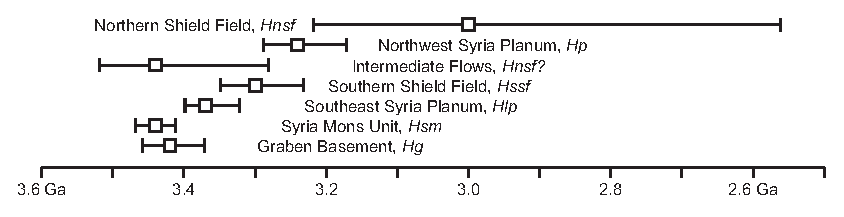
\includegraphics[width=1\textwidth]{figures/chapter-syria_planum/fig2.eps}
			\end{block}
			%% GNUPLOT: LaTeX picture
\setlength{\unitlength}{0.240900pt}
\ifx\plotpoint\undefined\newsavebox{\plotpoint}\fi
\sbox{\plotpoint}{\rule[-0.200pt]{0.400pt}{0.400pt}}%
\begin{picture}(1500,900)(0,0)
\sbox{\plotpoint}{\rule[-0.200pt]{0.400pt}{0.400pt}}%
\put(231.0,131.0){\rule[-0.200pt]{2.409pt}{0.400pt}}
\put(1429.0,131.0){\rule[-0.200pt]{2.409pt}{0.400pt}}
\put(231.0,169.0){\rule[-0.200pt]{2.409pt}{0.400pt}}
\put(1429.0,169.0){\rule[-0.200pt]{2.409pt}{0.400pt}}
\put(231.0,187.0){\rule[-0.200pt]{4.818pt}{0.400pt}}
\put(211,187){\makebox(0,0)[r]{ 1000}}
\put(1419.0,187.0){\rule[-0.200pt]{4.818pt}{0.400pt}}
\put(231.0,243.0){\rule[-0.200pt]{2.409pt}{0.400pt}}
\put(1429.0,243.0){\rule[-0.200pt]{2.409pt}{0.400pt}}
\put(231.0,318.0){\rule[-0.200pt]{2.409pt}{0.400pt}}
\put(1429.0,318.0){\rule[-0.200pt]{2.409pt}{0.400pt}}
\put(231.0,356.0){\rule[-0.200pt]{2.409pt}{0.400pt}}
\put(1429.0,356.0){\rule[-0.200pt]{2.409pt}{0.400pt}}
\put(231.0,374.0){\rule[-0.200pt]{4.818pt}{0.400pt}}
\put(211,374){\makebox(0,0)[r]{ 10000}}
\put(1419.0,374.0){\rule[-0.200pt]{4.818pt}{0.400pt}}
\put(231.0,430.0){\rule[-0.200pt]{2.409pt}{0.400pt}}
\put(1429.0,430.0){\rule[-0.200pt]{2.409pt}{0.400pt}}
\put(231.0,504.0){\rule[-0.200pt]{2.409pt}{0.400pt}}
\put(1429.0,504.0){\rule[-0.200pt]{2.409pt}{0.400pt}}
\put(231.0,542.0){\rule[-0.200pt]{2.409pt}{0.400pt}}
\put(1429.0,542.0){\rule[-0.200pt]{2.409pt}{0.400pt}}
\put(231.0,560.0){\rule[-0.200pt]{4.818pt}{0.400pt}}
\put(211,560){\makebox(0,0)[r]{ 100000}}
\put(1419.0,560.0){\rule[-0.200pt]{4.818pt}{0.400pt}}
\put(231.0,616.0){\rule[-0.200pt]{2.409pt}{0.400pt}}
\put(1429.0,616.0){\rule[-0.200pt]{2.409pt}{0.400pt}}
\put(231.0,691.0){\rule[-0.200pt]{2.409pt}{0.400pt}}
\put(1429.0,691.0){\rule[-0.200pt]{2.409pt}{0.400pt}}
\put(231.0,729.0){\rule[-0.200pt]{2.409pt}{0.400pt}}
\put(1429.0,729.0){\rule[-0.200pt]{2.409pt}{0.400pt}}
\put(231.0,747.0){\rule[-0.200pt]{4.818pt}{0.400pt}}
\put(211,747){\makebox(0,0)[r]{ 1e+06}}
\put(1419.0,747.0){\rule[-0.200pt]{4.818pt}{0.400pt}}
\put(231.0,803.0){\rule[-0.200pt]{2.409pt}{0.400pt}}
\put(1429.0,803.0){\rule[-0.200pt]{2.409pt}{0.400pt}}
\put(231.0,131.0){\rule[-0.200pt]{0.400pt}{2.409pt}}
\put(231.0,849.0){\rule[-0.200pt]{0.400pt}{2.409pt}}
\put(308.0,131.0){\rule[-0.200pt]{0.400pt}{2.409pt}}
\put(308.0,849.0){\rule[-0.200pt]{0.400pt}{2.409pt}}
\put(362.0,131.0){\rule[-0.200pt]{0.400pt}{2.409pt}}
\put(362.0,849.0){\rule[-0.200pt]{0.400pt}{2.409pt}}
\put(404.0,131.0){\rule[-0.200pt]{0.400pt}{2.409pt}}
\put(404.0,849.0){\rule[-0.200pt]{0.400pt}{2.409pt}}
\put(438.0,131.0){\rule[-0.200pt]{0.400pt}{2.409pt}}
\put(438.0,849.0){\rule[-0.200pt]{0.400pt}{2.409pt}}
\put(468.0,131.0){\rule[-0.200pt]{0.400pt}{2.409pt}}
\put(468.0,849.0){\rule[-0.200pt]{0.400pt}{2.409pt}}
\put(493.0,131.0){\rule[-0.200pt]{0.400pt}{2.409pt}}
\put(493.0,849.0){\rule[-0.200pt]{0.400pt}{2.409pt}}
\put(515.0,131.0){\rule[-0.200pt]{0.400pt}{2.409pt}}
\put(515.0,849.0){\rule[-0.200pt]{0.400pt}{2.409pt}}
\put(535.0,131.0){\rule[-0.200pt]{0.400pt}{4.818pt}}
\put(535,90){\makebox(0,0){ 100}}
\put(535.0,839.0){\rule[-0.200pt]{0.400pt}{4.818pt}}
\put(666.0,131.0){\rule[-0.200pt]{0.400pt}{2.409pt}}
\put(666.0,849.0){\rule[-0.200pt]{0.400pt}{2.409pt}}
\put(742.0,131.0){\rule[-0.200pt]{0.400pt}{2.409pt}}
\put(742.0,849.0){\rule[-0.200pt]{0.400pt}{2.409pt}}
\put(797.0,131.0){\rule[-0.200pt]{0.400pt}{2.409pt}}
\put(797.0,849.0){\rule[-0.200pt]{0.400pt}{2.409pt}}
\put(839.0,131.0){\rule[-0.200pt]{0.400pt}{2.409pt}}
\put(839.0,849.0){\rule[-0.200pt]{0.400pt}{2.409pt}}
\put(873.0,131.0){\rule[-0.200pt]{0.400pt}{2.409pt}}
\put(873.0,849.0){\rule[-0.200pt]{0.400pt}{2.409pt}}
\put(902.0,131.0){\rule[-0.200pt]{0.400pt}{2.409pt}}
\put(902.0,849.0){\rule[-0.200pt]{0.400pt}{2.409pt}}
\put(928.0,131.0){\rule[-0.200pt]{0.400pt}{2.409pt}}
\put(928.0,849.0){\rule[-0.200pt]{0.400pt}{2.409pt}}
\put(950.0,131.0){\rule[-0.200pt]{0.400pt}{2.409pt}}
\put(950.0,849.0){\rule[-0.200pt]{0.400pt}{2.409pt}}
\put(970.0,131.0){\rule[-0.200pt]{0.400pt}{4.818pt}}
\put(970,90){\makebox(0,0){ 1000}}
\put(970.0,839.0){\rule[-0.200pt]{0.400pt}{4.818pt}}
\put(1101.0,131.0){\rule[-0.200pt]{0.400pt}{2.409pt}}
\put(1101.0,849.0){\rule[-0.200pt]{0.400pt}{2.409pt}}
\put(1177.0,131.0){\rule[-0.200pt]{0.400pt}{2.409pt}}
\put(1177.0,849.0){\rule[-0.200pt]{0.400pt}{2.409pt}}
\put(1232.0,131.0){\rule[-0.200pt]{0.400pt}{2.409pt}}
\put(1232.0,849.0){\rule[-0.200pt]{0.400pt}{2.409pt}}
\put(1274.0,131.0){\rule[-0.200pt]{0.400pt}{2.409pt}}
\put(1274.0,849.0){\rule[-0.200pt]{0.400pt}{2.409pt}}
\put(1308.0,131.0){\rule[-0.200pt]{0.400pt}{2.409pt}}
\put(1308.0,849.0){\rule[-0.200pt]{0.400pt}{2.409pt}}
\put(1337.0,131.0){\rule[-0.200pt]{0.400pt}{2.409pt}}
\put(1337.0,849.0){\rule[-0.200pt]{0.400pt}{2.409pt}}
\put(1362.0,131.0){\rule[-0.200pt]{0.400pt}{2.409pt}}
\put(1362.0,849.0){\rule[-0.200pt]{0.400pt}{2.409pt}}
\put(1385.0,131.0){\rule[-0.200pt]{0.400pt}{2.409pt}}
\put(1385.0,849.0){\rule[-0.200pt]{0.400pt}{2.409pt}}
\put(1405.0,131.0){\rule[-0.200pt]{0.400pt}{4.818pt}}
\put(1405,90){\makebox(0,0){ 10000}}
\put(1405.0,839.0){\rule[-0.200pt]{0.400pt}{4.818pt}}
\put(231.0,131.0){\rule[-0.200pt]{0.400pt}{175.375pt}}
\put(231.0,131.0){\rule[-0.200pt]{291.007pt}{0.400pt}}
\put(1439.0,131.0){\rule[-0.200pt]{0.400pt}{175.375pt}}
\put(231.0,859.0){\rule[-0.200pt]{291.007pt}{0.400pt}}
\put(30,495){\rotatebox{-270}{\makebox(0,0){2-$sigma$ Cluster Size (km$^2$)}}
}\put(835,29){\makebox(0,0){Vent count in volcano cluster}}
\put(1046,374){\rotatebox{23}{\makebox(0,0)[l]{10 km$^2$ per vent}}
}\put(1046,560){\rotatebox{23}{\makebox(0,0)[l]{100 km$^2$ per vent}}
}\put(873,672){\rotatebox{23}{\makebox(0,0)[l]{1000 km$^2$ per vent}}
}\sbox{\plotpoint}{\rule[-0.500pt]{1.000pt}{1.000pt}}%
\multiput(404,131)(19.085,8.158){7}{\usebox{\plotpoint}}
\multiput(535,187)(19.068,8.197){23}{\usebox{\plotpoint}}
\multiput(970,374)(19.084,8.160){23}{\usebox{\plotpoint}}
\multiput(1405,560)(18.990,8.378){2}{\usebox{\plotpoint}}
\put(1439,575){\usebox{\plotpoint}}
\multiput(231,243)(19.061,8.214){16}{\usebox{\plotpoint}}
\multiput(535,374)(19.084,8.160){23}{\usebox{\plotpoint}}
\multiput(970,560)(19.068,8.197){23}{\usebox{\plotpoint}}
\multiput(1405,747)(19.192,7.903){2}{\usebox{\plotpoint}}
\put(1439,761){\usebox{\plotpoint}}
\multiput(231,430)(19.084,8.161){16}{\usebox{\plotpoint}}
\multiput(535,560)(19.068,8.197){23}{\usebox{\plotpoint}}
\multiput(970,747)(19.085,8.158){14}{\usebox{\plotpoint}}
\put(1232,859){\usebox{\plotpoint}}
\sbox{\plotpoint}{\rule[-0.200pt]{0.400pt}{0.400pt}}%
\put(571,819){\makebox(0,0)[r]{  Earth Clusters}}
\sbox{\plotpoint}{\rule[-0.500pt]{1.000pt}{1.000pt}}%
\put(486,188){\makebox(0,0){$\circ$}}
\put(868,324){\makebox(0,0){$\circ$}}
\put(448,180){\makebox(0,0){$\circ$}}
\put(793,259){\makebox(0,0){$\circ$}}
\put(513,194){\makebox(0,0){$\circ$}}
\put(758,233){\makebox(0,0){$\circ$}}
\put(641,819){\makebox(0,0){$\circ$}}
\sbox{\plotpoint}{\rule[-0.600pt]{1.200pt}{1.200pt}}%
\sbox{\plotpoint}{\rule[-0.200pt]{0.400pt}{0.400pt}}%
\put(571,778){\makebox(0,0)[r]{  Venus Clusters}}
\sbox{\plotpoint}{\rule[-0.600pt]{1.200pt}{1.200pt}}%
\put(767,467){\makebox(0,0){$\bullet$}}
\put(590,364){\makebox(0,0){$\bullet$}}
\put(633,404){\makebox(0,0){$\bullet$}}
\put(735,426){\makebox(0,0){$\bullet$}}
\put(1169,751){\makebox(0,0){$\bullet$}}
\put(1405,777){\makebox(0,0){$\bullet$}}
\put(1201,746){\makebox(0,0){$\bullet$}}
\put(641,778){\makebox(0,0){$\bullet$}}
\sbox{\plotpoint}{\rule[-0.500pt]{1.000pt}{1.000pt}}%
\sbox{\plotpoint}{\rule[-0.200pt]{0.400pt}{0.400pt}}%
\put(571,737){\makebox(0,0)[r]{  Mars Clusters}}
\sbox{\plotpoint}{\rule[-0.500pt]{1.000pt}{1.000pt}}%
\put(301,376){\makebox(0,0){$\ast$}}
\put(513,574){\makebox(0,0){$\ast$}}
\put(715,656){\makebox(0,0){$\ast$}}
\put(641,737){\makebox(0,0){$\ast$}}
\sbox{\plotpoint}{\rule[-0.200pt]{0.400pt}{0.400pt}}%
\put(231.0,131.0){\rule[-0.200pt]{0.400pt}{175.375pt}}
\put(231.0,131.0){\rule[-0.200pt]{291.007pt}{0.400pt}}
\put(1439.0,131.0){\rule[-0.200pt]{0.400pt}{175.375pt}}
\put(231.0,859.0){\rule[-0.200pt]{291.007pt}{0.400pt}}
\end{picture}

		\end{columns}
	}

	\frame{\frametitle{Syria Planum}
		\begin{columns}
		\column{.46\textwidth}
			\centering
			\includegraphics[width=1\textwidth,clip,trim=1cm 5cm 1cm 1mm]{figures/chapter-syria_planum/fig1.eps}
		\column{.54\textwidth}
			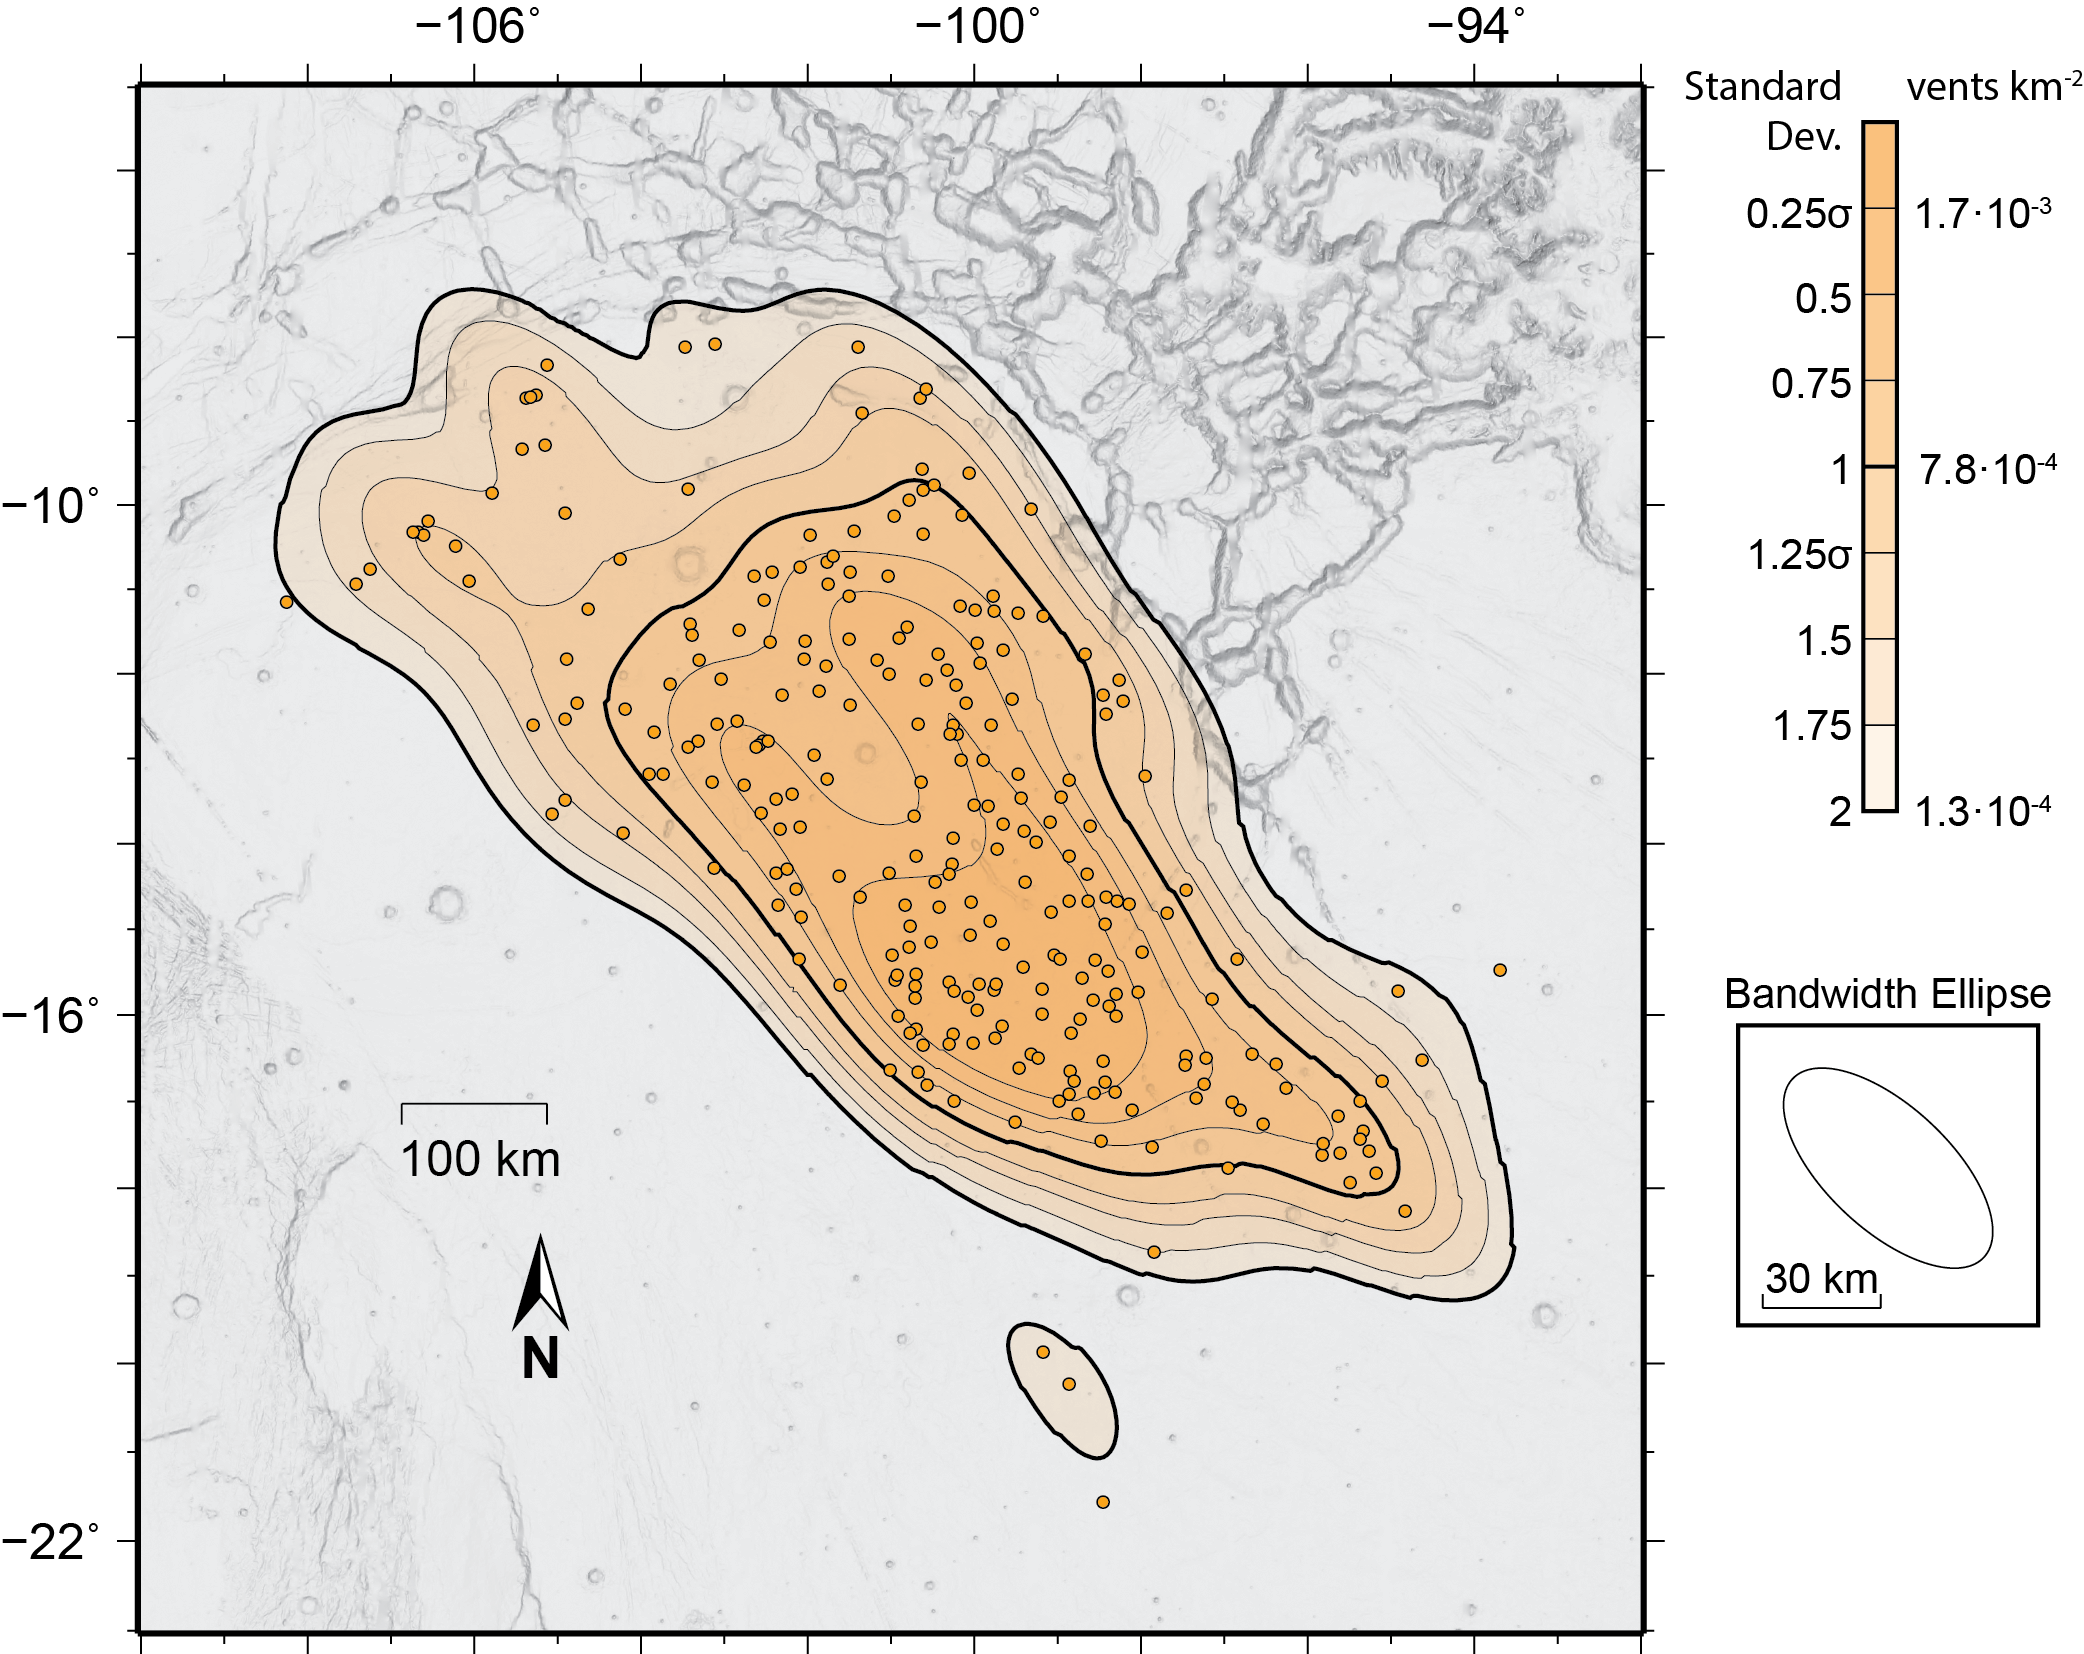
\includegraphics[width=1\textwidth]{figures/chapter-spatial_density/syria_kde_300dpi.png}
			%% GNUPLOT: LaTeX picture
\setlength{\unitlength}{0.240900pt}
\ifx\plotpoint\undefined\newsavebox{\plotpoint}\fi
\sbox{\plotpoint}{\rule[-0.200pt]{0.400pt}{0.400pt}}%
\begin{picture}(1500,900)(0,0)
\sbox{\plotpoint}{\rule[-0.200pt]{0.400pt}{0.400pt}}%
\put(231.0,131.0){\rule[-0.200pt]{2.409pt}{0.400pt}}
\put(1429.0,131.0){\rule[-0.200pt]{2.409pt}{0.400pt}}
\put(231.0,169.0){\rule[-0.200pt]{2.409pt}{0.400pt}}
\put(1429.0,169.0){\rule[-0.200pt]{2.409pt}{0.400pt}}
\put(231.0,187.0){\rule[-0.200pt]{4.818pt}{0.400pt}}
\put(211,187){\makebox(0,0)[r]{ 1000}}
\put(1419.0,187.0){\rule[-0.200pt]{4.818pt}{0.400pt}}
\put(231.0,243.0){\rule[-0.200pt]{2.409pt}{0.400pt}}
\put(1429.0,243.0){\rule[-0.200pt]{2.409pt}{0.400pt}}
\put(231.0,318.0){\rule[-0.200pt]{2.409pt}{0.400pt}}
\put(1429.0,318.0){\rule[-0.200pt]{2.409pt}{0.400pt}}
\put(231.0,356.0){\rule[-0.200pt]{2.409pt}{0.400pt}}
\put(1429.0,356.0){\rule[-0.200pt]{2.409pt}{0.400pt}}
\put(231.0,374.0){\rule[-0.200pt]{4.818pt}{0.400pt}}
\put(211,374){\makebox(0,0)[r]{ 10000}}
\put(1419.0,374.0){\rule[-0.200pt]{4.818pt}{0.400pt}}
\put(231.0,430.0){\rule[-0.200pt]{2.409pt}{0.400pt}}
\put(1429.0,430.0){\rule[-0.200pt]{2.409pt}{0.400pt}}
\put(231.0,504.0){\rule[-0.200pt]{2.409pt}{0.400pt}}
\put(1429.0,504.0){\rule[-0.200pt]{2.409pt}{0.400pt}}
\put(231.0,542.0){\rule[-0.200pt]{2.409pt}{0.400pt}}
\put(1429.0,542.0){\rule[-0.200pt]{2.409pt}{0.400pt}}
\put(231.0,560.0){\rule[-0.200pt]{4.818pt}{0.400pt}}
\put(211,560){\makebox(0,0)[r]{ 100000}}
\put(1419.0,560.0){\rule[-0.200pt]{4.818pt}{0.400pt}}
\put(231.0,616.0){\rule[-0.200pt]{2.409pt}{0.400pt}}
\put(1429.0,616.0){\rule[-0.200pt]{2.409pt}{0.400pt}}
\put(231.0,691.0){\rule[-0.200pt]{2.409pt}{0.400pt}}
\put(1429.0,691.0){\rule[-0.200pt]{2.409pt}{0.400pt}}
\put(231.0,729.0){\rule[-0.200pt]{2.409pt}{0.400pt}}
\put(1429.0,729.0){\rule[-0.200pt]{2.409pt}{0.400pt}}
\put(231.0,747.0){\rule[-0.200pt]{4.818pt}{0.400pt}}
\put(211,747){\makebox(0,0)[r]{ 1e+06}}
\put(1419.0,747.0){\rule[-0.200pt]{4.818pt}{0.400pt}}
\put(231.0,803.0){\rule[-0.200pt]{2.409pt}{0.400pt}}
\put(1429.0,803.0){\rule[-0.200pt]{2.409pt}{0.400pt}}
\put(231.0,131.0){\rule[-0.200pt]{0.400pt}{2.409pt}}
\put(231.0,849.0){\rule[-0.200pt]{0.400pt}{2.409pt}}
\put(308.0,131.0){\rule[-0.200pt]{0.400pt}{2.409pt}}
\put(308.0,849.0){\rule[-0.200pt]{0.400pt}{2.409pt}}
\put(362.0,131.0){\rule[-0.200pt]{0.400pt}{2.409pt}}
\put(362.0,849.0){\rule[-0.200pt]{0.400pt}{2.409pt}}
\put(404.0,131.0){\rule[-0.200pt]{0.400pt}{2.409pt}}
\put(404.0,849.0){\rule[-0.200pt]{0.400pt}{2.409pt}}
\put(438.0,131.0){\rule[-0.200pt]{0.400pt}{2.409pt}}
\put(438.0,849.0){\rule[-0.200pt]{0.400pt}{2.409pt}}
\put(468.0,131.0){\rule[-0.200pt]{0.400pt}{2.409pt}}
\put(468.0,849.0){\rule[-0.200pt]{0.400pt}{2.409pt}}
\put(493.0,131.0){\rule[-0.200pt]{0.400pt}{2.409pt}}
\put(493.0,849.0){\rule[-0.200pt]{0.400pt}{2.409pt}}
\put(515.0,131.0){\rule[-0.200pt]{0.400pt}{2.409pt}}
\put(515.0,849.0){\rule[-0.200pt]{0.400pt}{2.409pt}}
\put(535.0,131.0){\rule[-0.200pt]{0.400pt}{4.818pt}}
\put(535,90){\makebox(0,0){ 100}}
\put(535.0,839.0){\rule[-0.200pt]{0.400pt}{4.818pt}}
\put(666.0,131.0){\rule[-0.200pt]{0.400pt}{2.409pt}}
\put(666.0,849.0){\rule[-0.200pt]{0.400pt}{2.409pt}}
\put(742.0,131.0){\rule[-0.200pt]{0.400pt}{2.409pt}}
\put(742.0,849.0){\rule[-0.200pt]{0.400pt}{2.409pt}}
\put(797.0,131.0){\rule[-0.200pt]{0.400pt}{2.409pt}}
\put(797.0,849.0){\rule[-0.200pt]{0.400pt}{2.409pt}}
\put(839.0,131.0){\rule[-0.200pt]{0.400pt}{2.409pt}}
\put(839.0,849.0){\rule[-0.200pt]{0.400pt}{2.409pt}}
\put(873.0,131.0){\rule[-0.200pt]{0.400pt}{2.409pt}}
\put(873.0,849.0){\rule[-0.200pt]{0.400pt}{2.409pt}}
\put(902.0,131.0){\rule[-0.200pt]{0.400pt}{2.409pt}}
\put(902.0,849.0){\rule[-0.200pt]{0.400pt}{2.409pt}}
\put(928.0,131.0){\rule[-0.200pt]{0.400pt}{2.409pt}}
\put(928.0,849.0){\rule[-0.200pt]{0.400pt}{2.409pt}}
\put(950.0,131.0){\rule[-0.200pt]{0.400pt}{2.409pt}}
\put(950.0,849.0){\rule[-0.200pt]{0.400pt}{2.409pt}}
\put(970.0,131.0){\rule[-0.200pt]{0.400pt}{4.818pt}}
\put(970,90){\makebox(0,0){ 1000}}
\put(970.0,839.0){\rule[-0.200pt]{0.400pt}{4.818pt}}
\put(1101.0,131.0){\rule[-0.200pt]{0.400pt}{2.409pt}}
\put(1101.0,849.0){\rule[-0.200pt]{0.400pt}{2.409pt}}
\put(1177.0,131.0){\rule[-0.200pt]{0.400pt}{2.409pt}}
\put(1177.0,849.0){\rule[-0.200pt]{0.400pt}{2.409pt}}
\put(1232.0,131.0){\rule[-0.200pt]{0.400pt}{2.409pt}}
\put(1232.0,849.0){\rule[-0.200pt]{0.400pt}{2.409pt}}
\put(1274.0,131.0){\rule[-0.200pt]{0.400pt}{2.409pt}}
\put(1274.0,849.0){\rule[-0.200pt]{0.400pt}{2.409pt}}
\put(1308.0,131.0){\rule[-0.200pt]{0.400pt}{2.409pt}}
\put(1308.0,849.0){\rule[-0.200pt]{0.400pt}{2.409pt}}
\put(1337.0,131.0){\rule[-0.200pt]{0.400pt}{2.409pt}}
\put(1337.0,849.0){\rule[-0.200pt]{0.400pt}{2.409pt}}
\put(1362.0,131.0){\rule[-0.200pt]{0.400pt}{2.409pt}}
\put(1362.0,849.0){\rule[-0.200pt]{0.400pt}{2.409pt}}
\put(1385.0,131.0){\rule[-0.200pt]{0.400pt}{2.409pt}}
\put(1385.0,849.0){\rule[-0.200pt]{0.400pt}{2.409pt}}
\put(1405.0,131.0){\rule[-0.200pt]{0.400pt}{4.818pt}}
\put(1405,90){\makebox(0,0){ 10000}}
\put(1405.0,839.0){\rule[-0.200pt]{0.400pt}{4.818pt}}
\put(231.0,131.0){\rule[-0.200pt]{0.400pt}{175.375pt}}
\put(231.0,131.0){\rule[-0.200pt]{291.007pt}{0.400pt}}
\put(1439.0,131.0){\rule[-0.200pt]{0.400pt}{175.375pt}}
\put(231.0,859.0){\rule[-0.200pt]{291.007pt}{0.400pt}}
\put(30,495){\rotatebox{-270}{\makebox(0,0){2-$sigma$ Cluster Size (km$^2$)}}
}\put(835,29){\makebox(0,0){Vent count in volcano cluster}}
\put(1046,374){\rotatebox{23}{\makebox(0,0)[l]{10 km$^2$ per vent}}
}\put(1046,560){\rotatebox{23}{\makebox(0,0)[l]{100 km$^2$ per vent}}
}\put(873,672){\rotatebox{23}{\makebox(0,0)[l]{1000 km$^2$ per vent}}
}\sbox{\plotpoint}{\rule[-0.500pt]{1.000pt}{1.000pt}}%
\multiput(404,131)(19.085,8.158){7}{\usebox{\plotpoint}}
\multiput(535,187)(19.068,8.197){23}{\usebox{\plotpoint}}
\multiput(970,374)(19.084,8.160){23}{\usebox{\plotpoint}}
\multiput(1405,560)(18.990,8.378){2}{\usebox{\plotpoint}}
\put(1439,575){\usebox{\plotpoint}}
\multiput(231,243)(19.061,8.214){16}{\usebox{\plotpoint}}
\multiput(535,374)(19.084,8.160){23}{\usebox{\plotpoint}}
\multiput(970,560)(19.068,8.197){23}{\usebox{\plotpoint}}
\multiput(1405,747)(19.192,7.903){2}{\usebox{\plotpoint}}
\put(1439,761){\usebox{\plotpoint}}
\multiput(231,430)(19.084,8.161){16}{\usebox{\plotpoint}}
\multiput(535,560)(19.068,8.197){23}{\usebox{\plotpoint}}
\multiput(970,747)(19.085,8.158){14}{\usebox{\plotpoint}}
\put(1232,859){\usebox{\plotpoint}}
\sbox{\plotpoint}{\rule[-0.200pt]{0.400pt}{0.400pt}}%
\put(571,819){\makebox(0,0)[r]{  Earth Clusters}}
\sbox{\plotpoint}{\rule[-0.500pt]{1.000pt}{1.000pt}}%
\put(486,188){\makebox(0,0){$\circ$}}
\put(868,324){\makebox(0,0){$\circ$}}
\put(448,180){\makebox(0,0){$\circ$}}
\put(793,259){\makebox(0,0){$\circ$}}
\put(513,194){\makebox(0,0){$\circ$}}
\put(758,233){\makebox(0,0){$\circ$}}
\put(641,819){\makebox(0,0){$\circ$}}
\sbox{\plotpoint}{\rule[-0.600pt]{1.200pt}{1.200pt}}%
\sbox{\plotpoint}{\rule[-0.200pt]{0.400pt}{0.400pt}}%
\put(571,778){\makebox(0,0)[r]{  Venus Clusters}}
\sbox{\plotpoint}{\rule[-0.600pt]{1.200pt}{1.200pt}}%
\put(767,467){\makebox(0,0){$\bullet$}}
\put(590,364){\makebox(0,0){$\bullet$}}
\put(633,404){\makebox(0,0){$\bullet$}}
\put(735,426){\makebox(0,0){$\bullet$}}
\put(1169,751){\makebox(0,0){$\bullet$}}
\put(1405,777){\makebox(0,0){$\bullet$}}
\put(1201,746){\makebox(0,0){$\bullet$}}
\put(641,778){\makebox(0,0){$\bullet$}}
\sbox{\plotpoint}{\rule[-0.500pt]{1.000pt}{1.000pt}}%
\sbox{\plotpoint}{\rule[-0.200pt]{0.400pt}{0.400pt}}%
\put(571,737){\makebox(0,0)[r]{  Mars Clusters}}
\sbox{\plotpoint}{\rule[-0.500pt]{1.000pt}{1.000pt}}%
\put(301,376){\makebox(0,0){$\ast$}}
\put(513,574){\makebox(0,0){$\ast$}}
\put(715,656){\makebox(0,0){$\ast$}}
\put(641,737){\makebox(0,0){$\ast$}}
\sbox{\plotpoint}{\rule[-0.200pt]{0.400pt}{0.400pt}}%
\put(231.0,131.0){\rule[-0.200pt]{0.400pt}{175.375pt}}
\put(231.0,131.0){\rule[-0.200pt]{291.007pt}{0.400pt}}
\put(1439.0,131.0){\rule[-0.200pt]{0.400pt}{175.375pt}}
\put(231.0,859.0){\rule[-0.200pt]{291.007pt}{0.400pt}}
\end{picture}

		\end{columns}
	}

%%%%%%%%%%%%%%%%%%%%%%%%%%%%%%%%%%%%%%%%%%%%%%%%%%%%%%%%%%
%%   ARSIA MONS   %%
%%%%%%%%%%%%%%%%%%%%%%%%%%%%%%%%%%%%%%%
%%%%%%%%%%%%%%%%%%%%%%%%%%%%%%
%%%%%%%%%%%%%%%%%%%%%
%%%%%%%%%%%%

\section{Arsia Mons Volcanic Field}
	\frame{\frametitle{Arsia Mons: An introduction}
		\begin{block}{}
		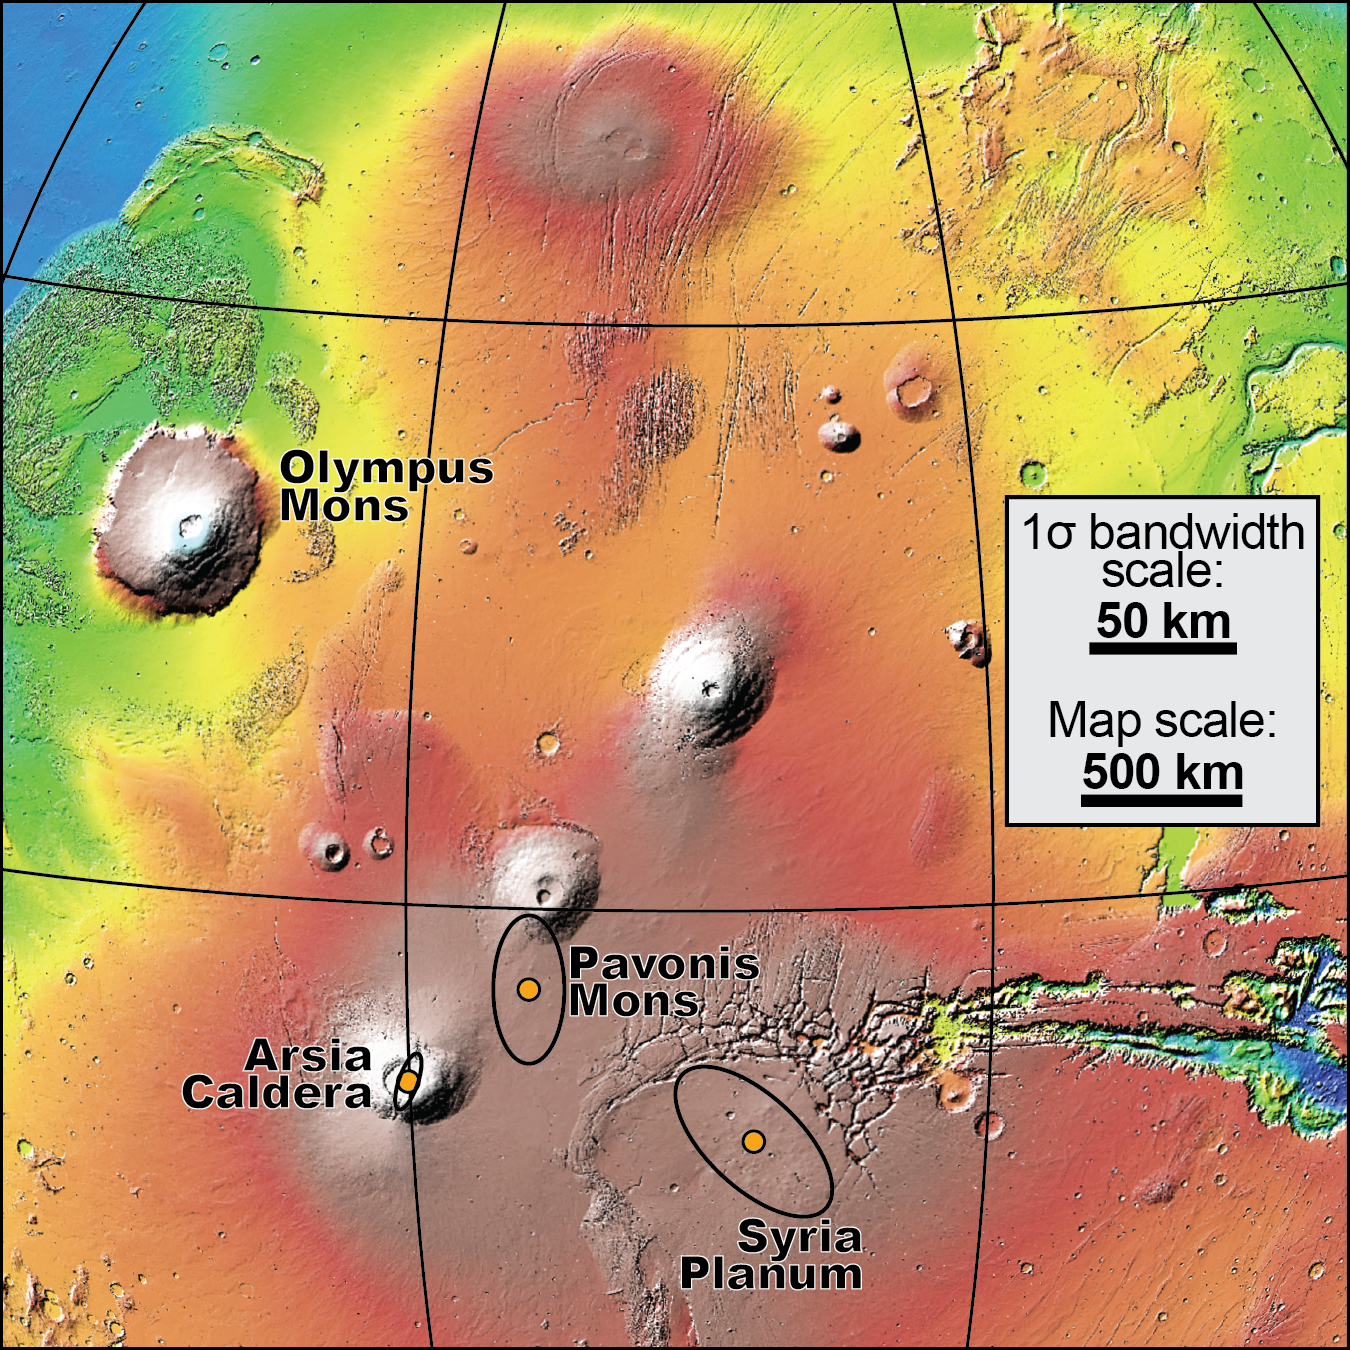
\includegraphics[width=0.8\textwidth]{figures/defense/mars_locator_300dpi}
		\end{block}
	}

\subsection{Methods}
	\frame{\frametitle{Mapping}
		\begin{block}{}
		%Change to just the outlines.
		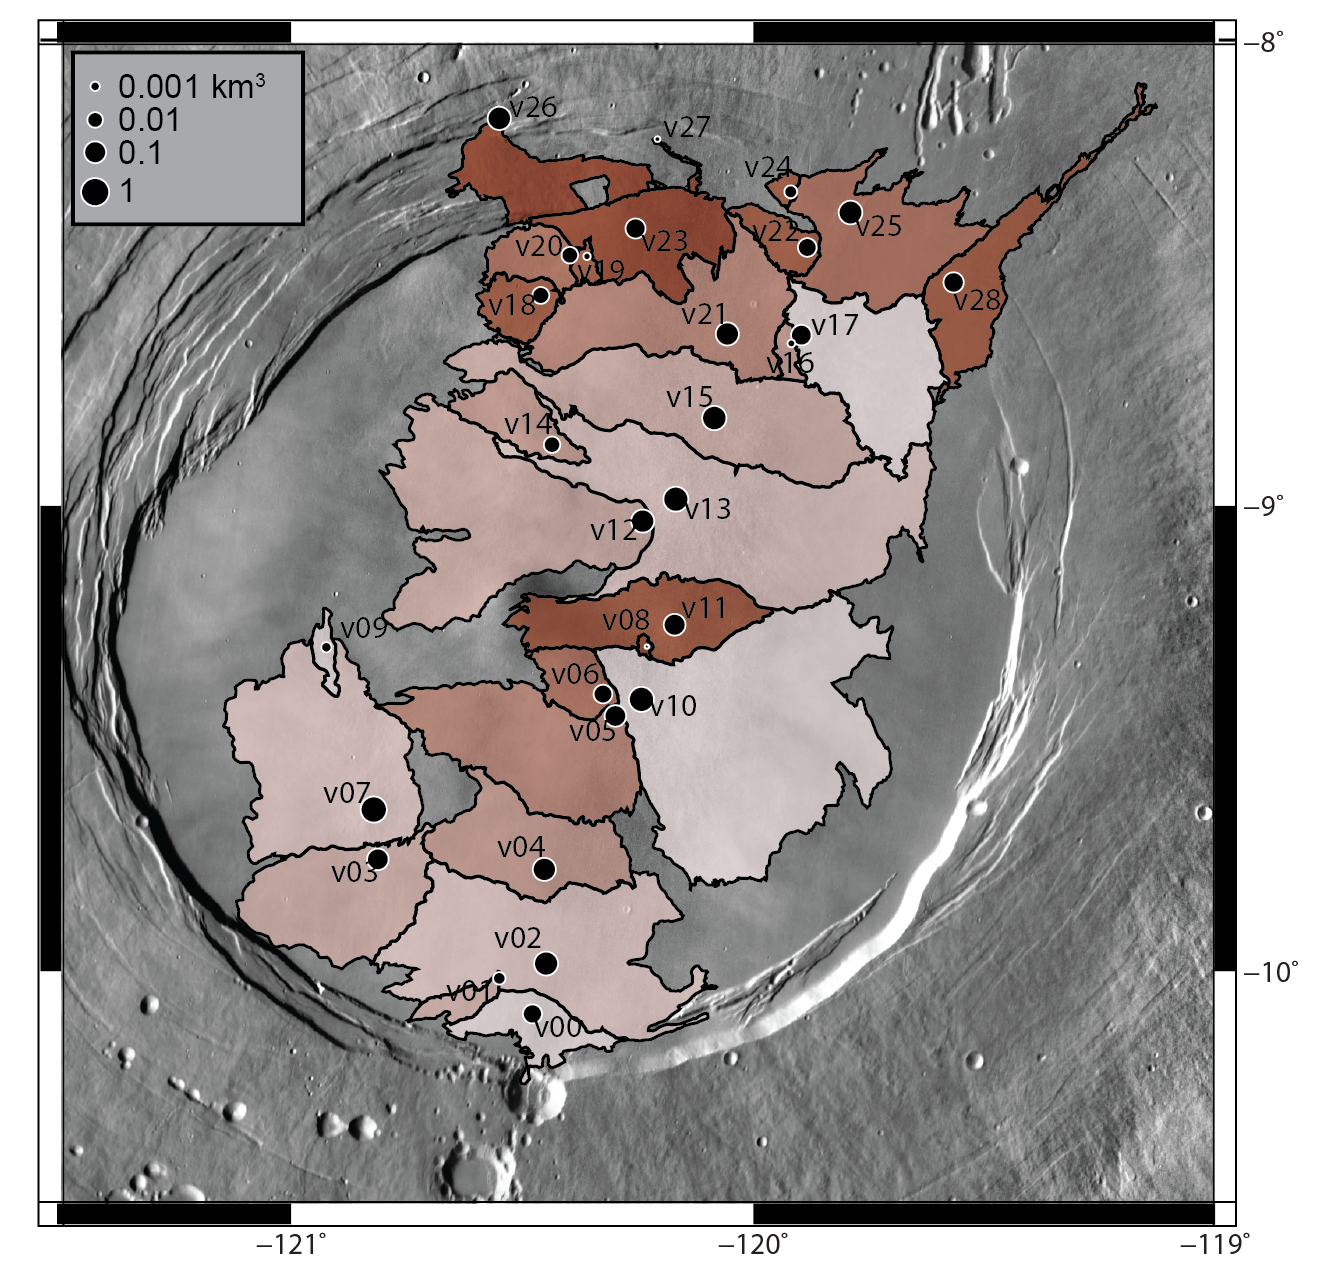
\includegraphics[width=0.8\textwidth]{figures/chapter-arsia/vent_map-01.png}
		%Examples
		\end{block}
	}

	\frame{\frametitle{Volume}
	%Mola MIN
	%Thicknesses
	}

	\frame{\frametitle{Ages: Crater Counting}
	%Crater Stats 2
	%Examples:
	%V10 - 120.24W_09.42W
	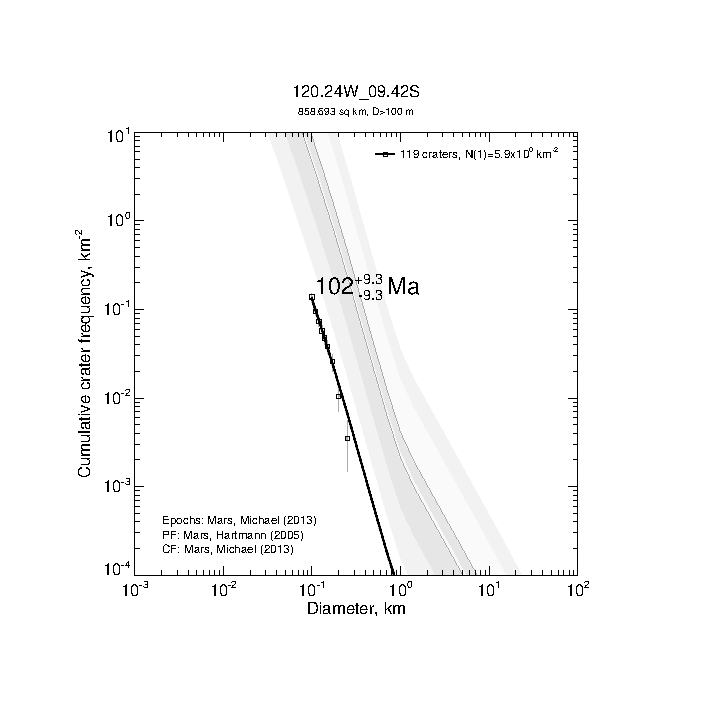
\includegraphics[width=0.3\textwidth]{figures/chapter-arsia/craterstats/120-24W_09-42S_100m_cum.eps}
	}
	
	\frame{\frametitle{Ages: Crater Counting}
	%Uncertainty Discussion
	%Cumulative Function
	%PDF
	%Assumes constant impact crater formation rate to be Gaussian
	}

	\frame{\frametitle{Ages: Stratigraphy}
	%Examples
	%Stratigraphy Web Key
	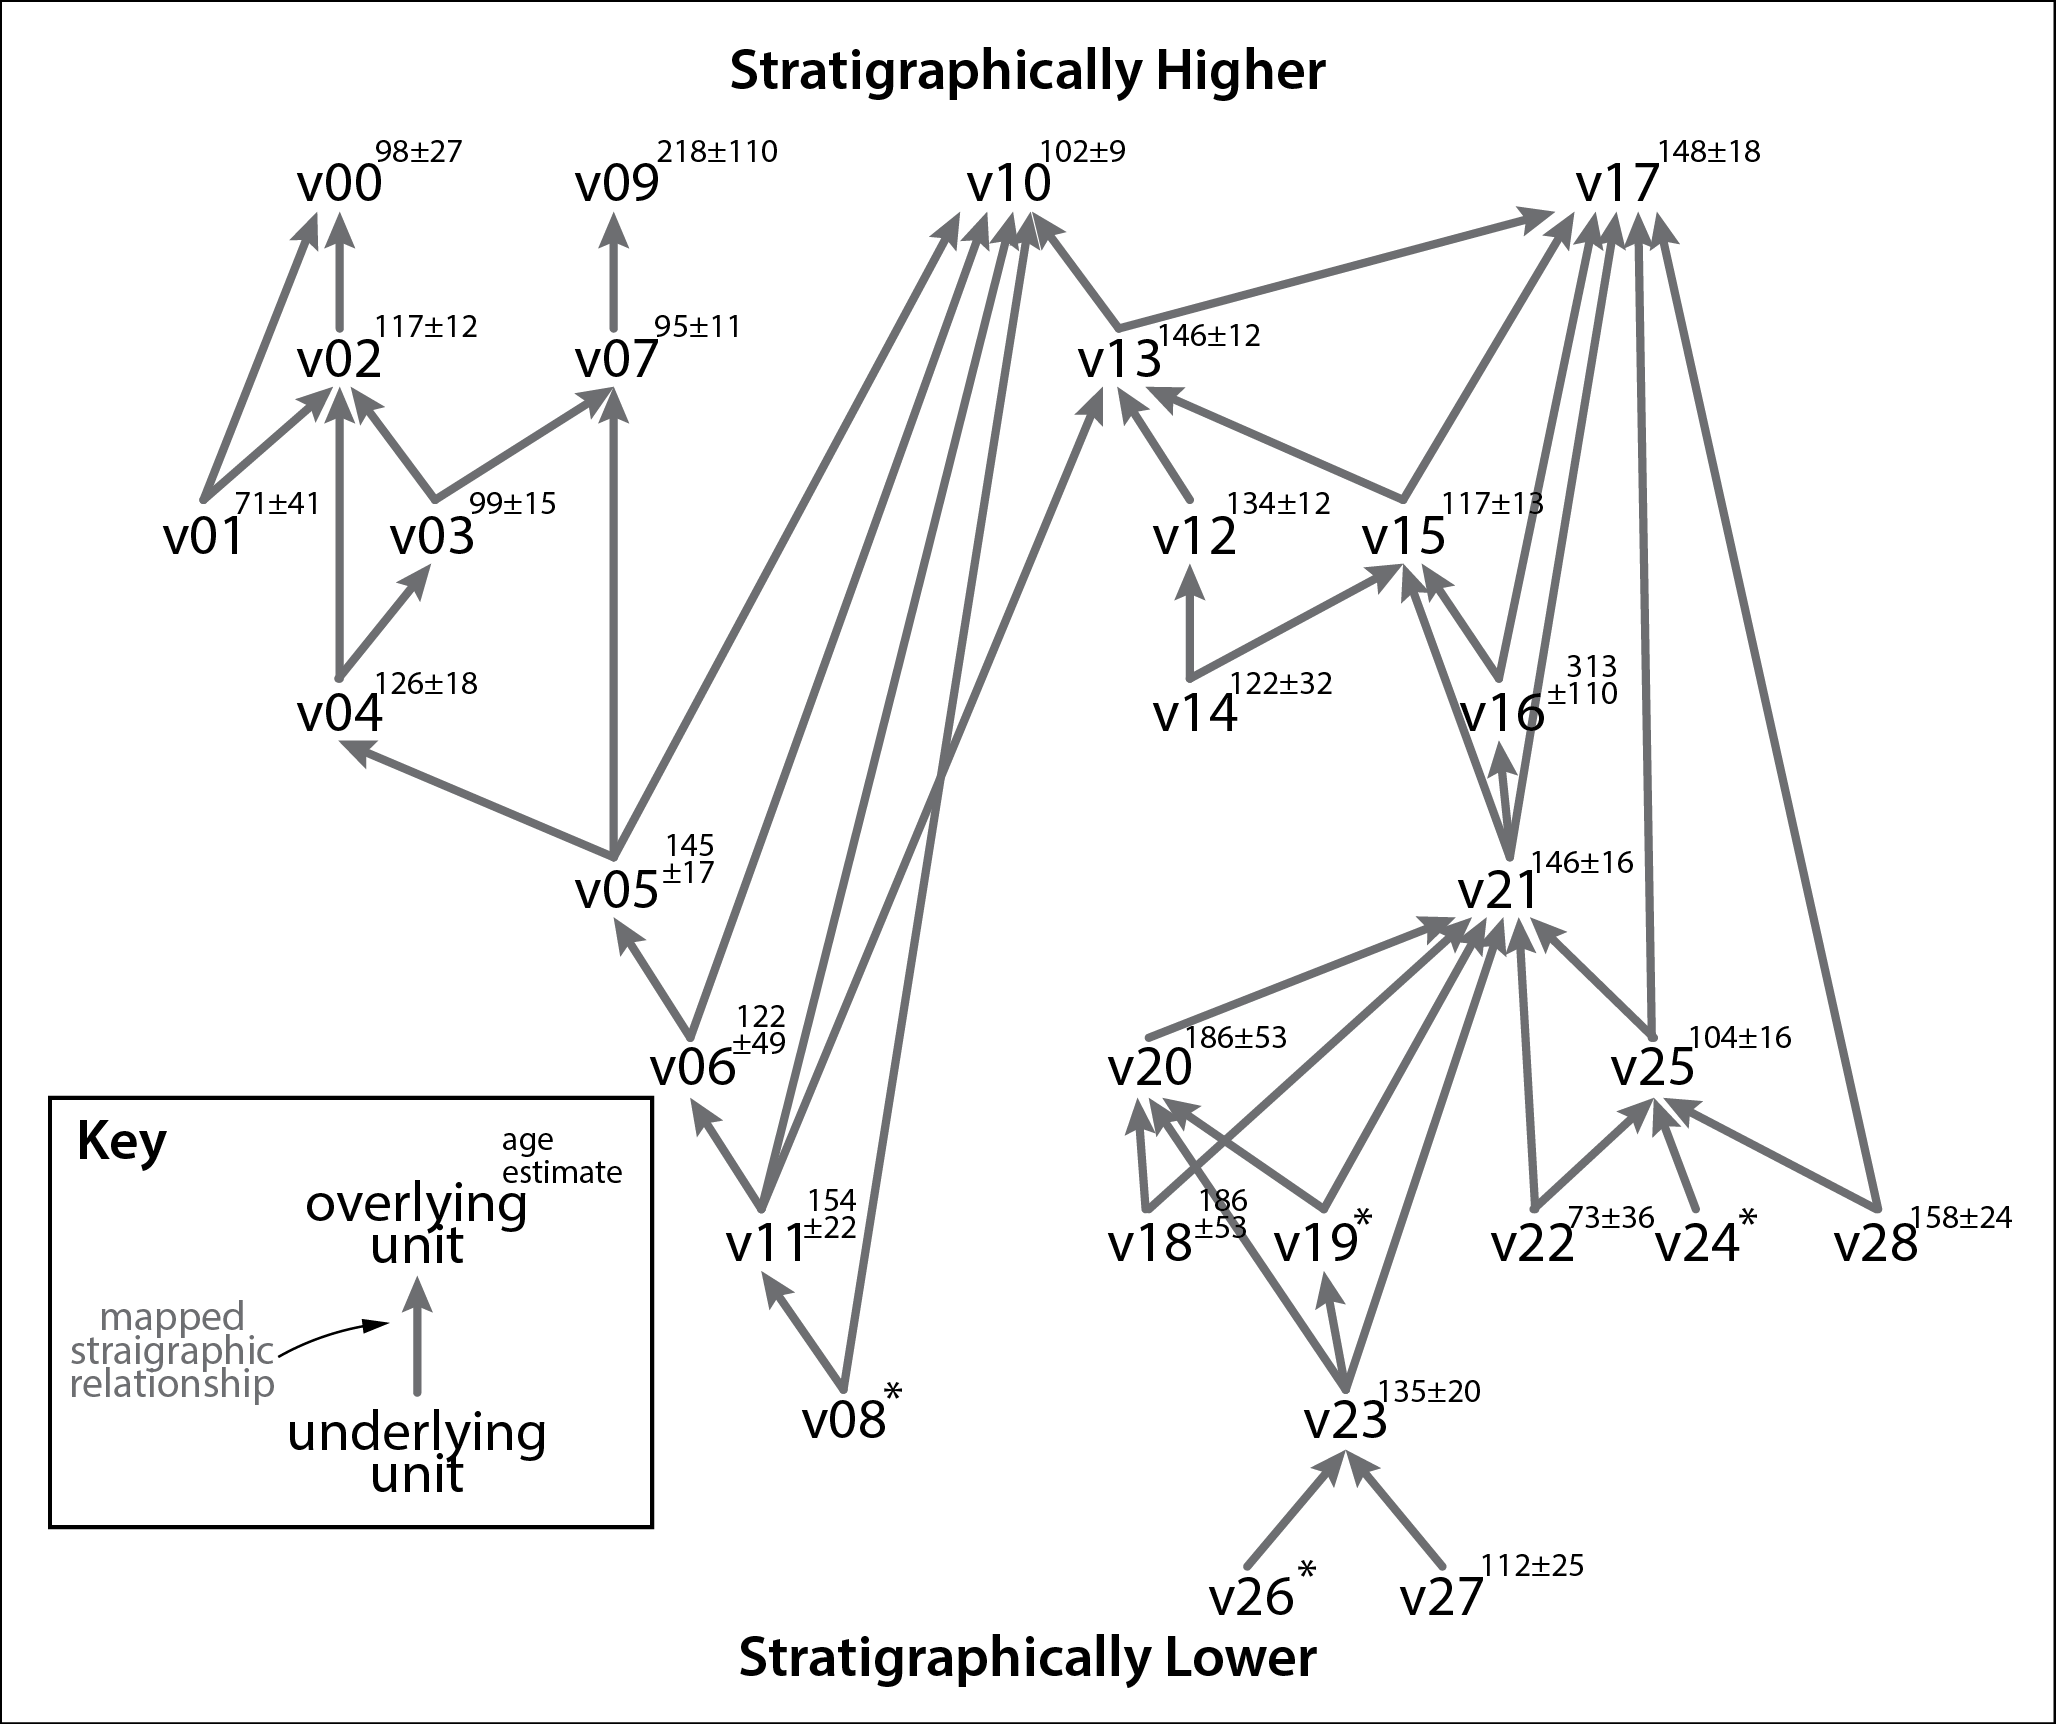
\includegraphics[width=0.3\textwidth,clip,trim=0.2cm 1cm 11.8cm 9.2cm]{figures/chapter-arsia/stratigraphy_web_300dpi.png} %
	}

	\frame{\frametitle{Ages}
	%Stratigraphy Web
	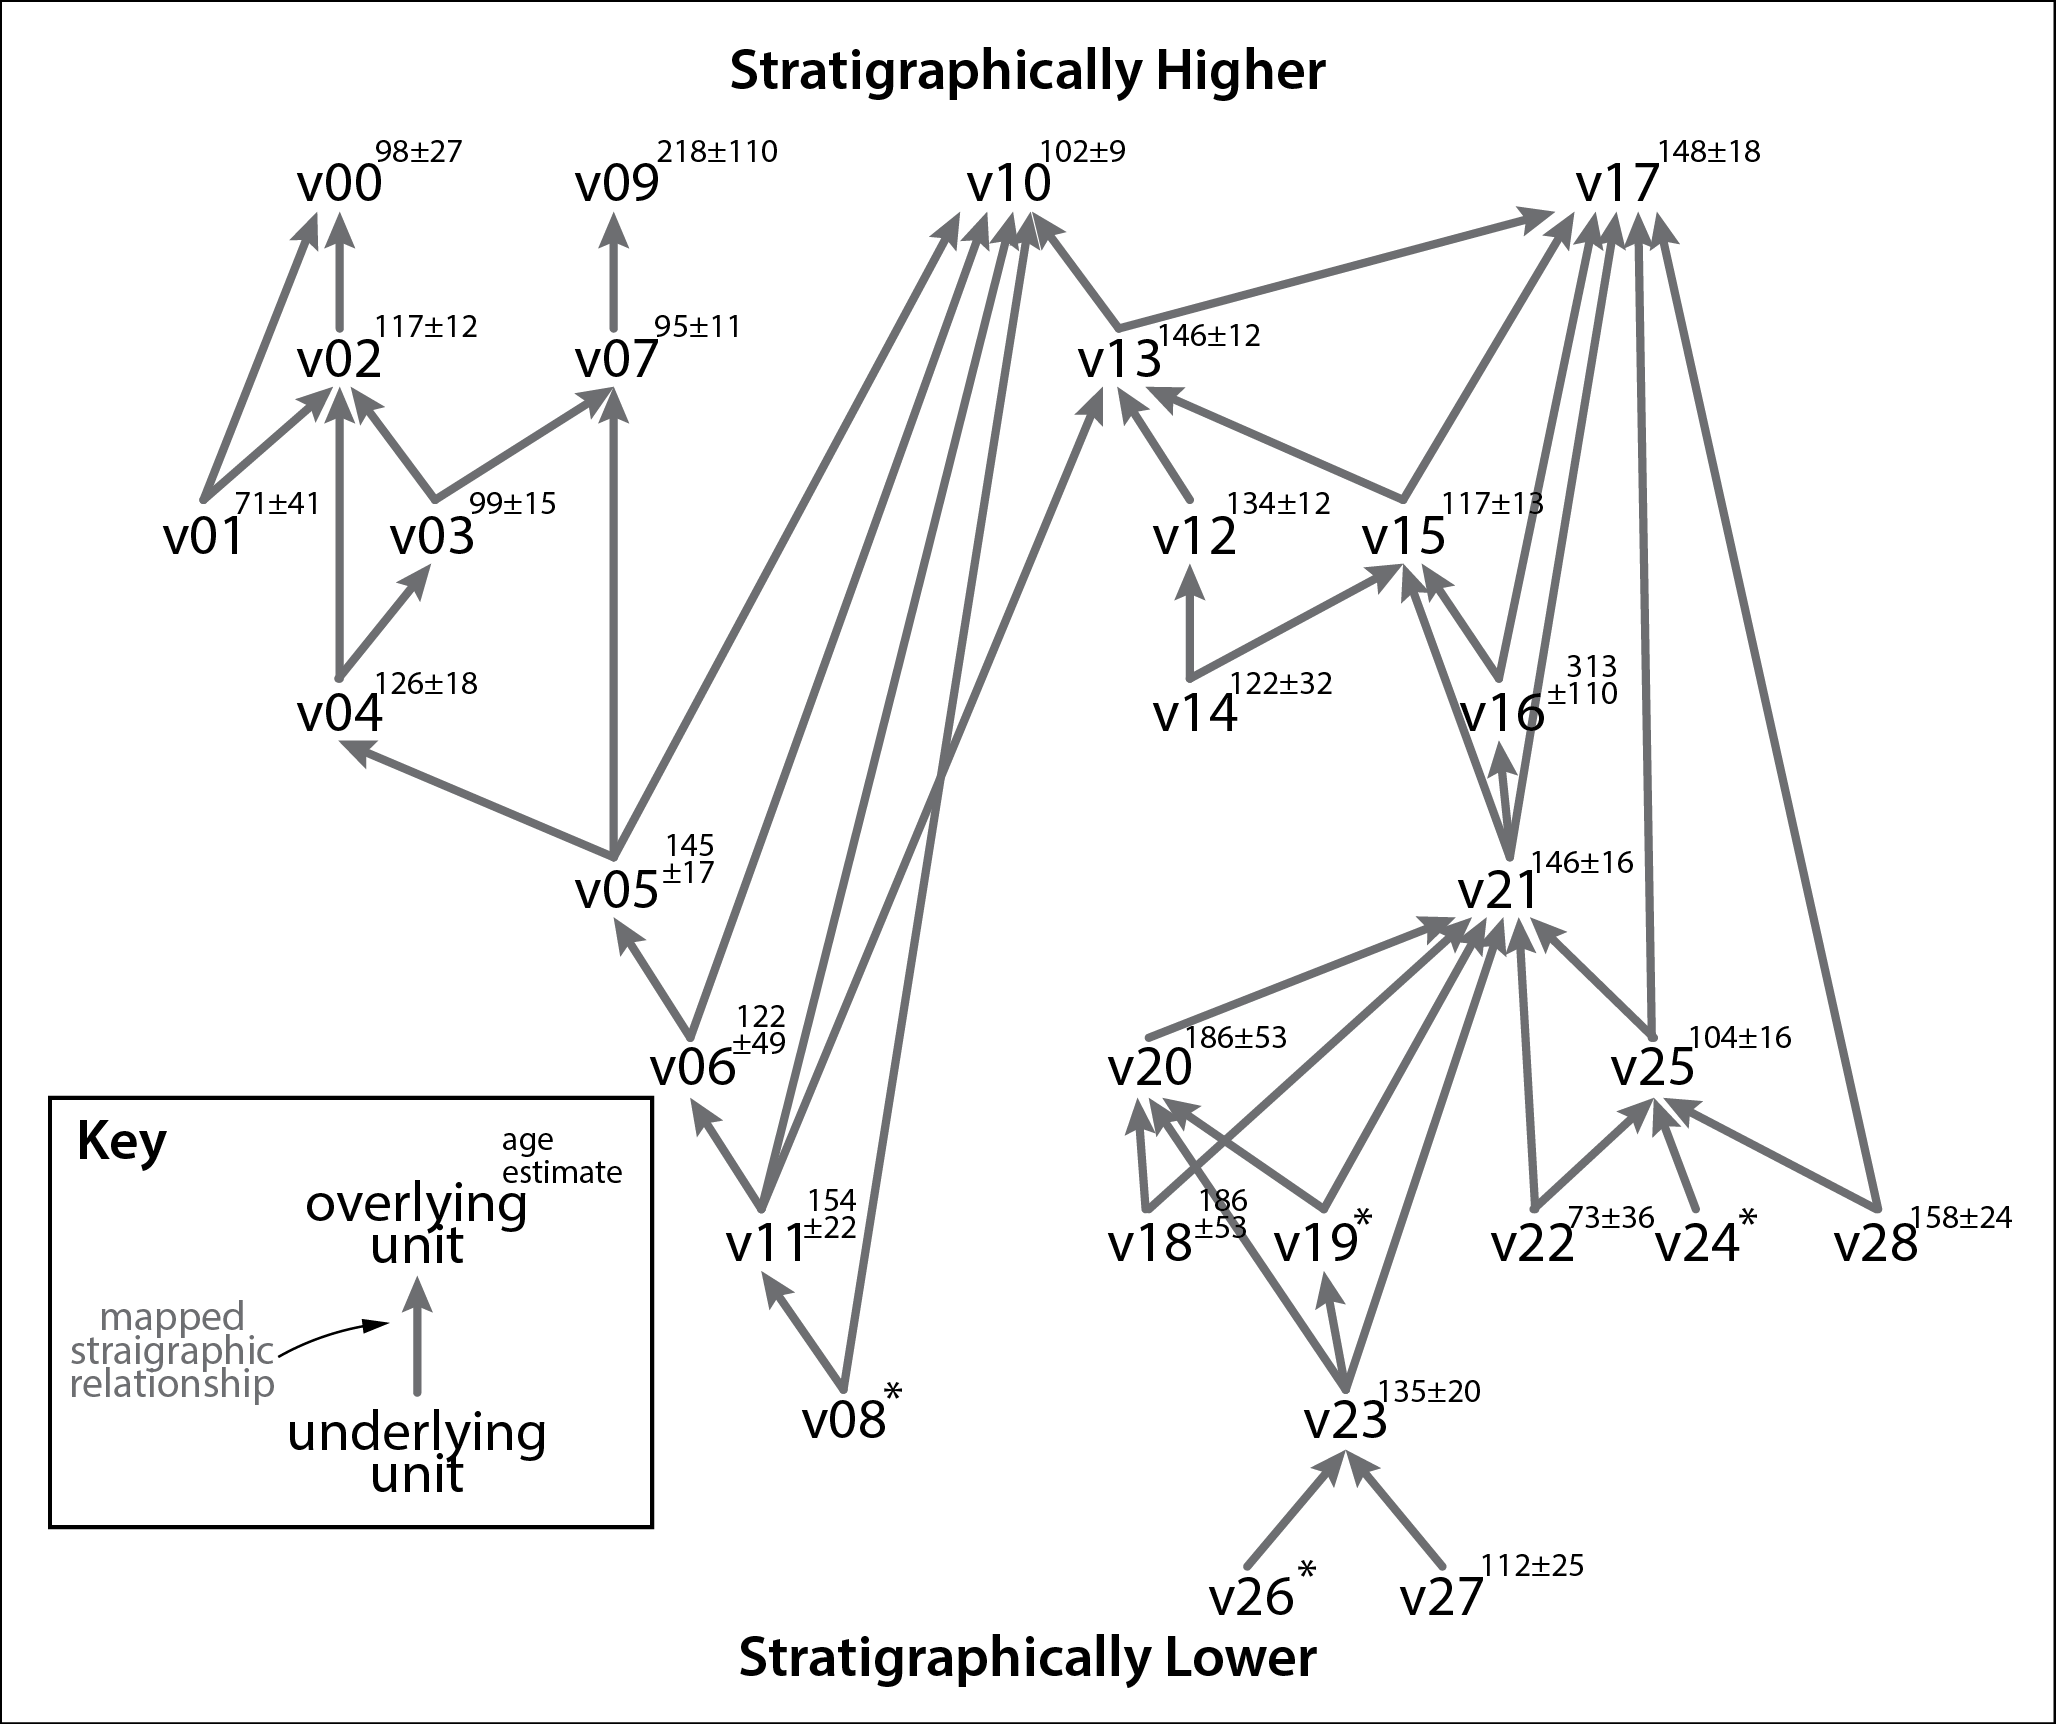
\includegraphics[width=0.5\textwidth]{figures/chapter-arsia/stratigraphy_web_300dpi.png}
	%Stratigraphy Map - Change to get rid of 
	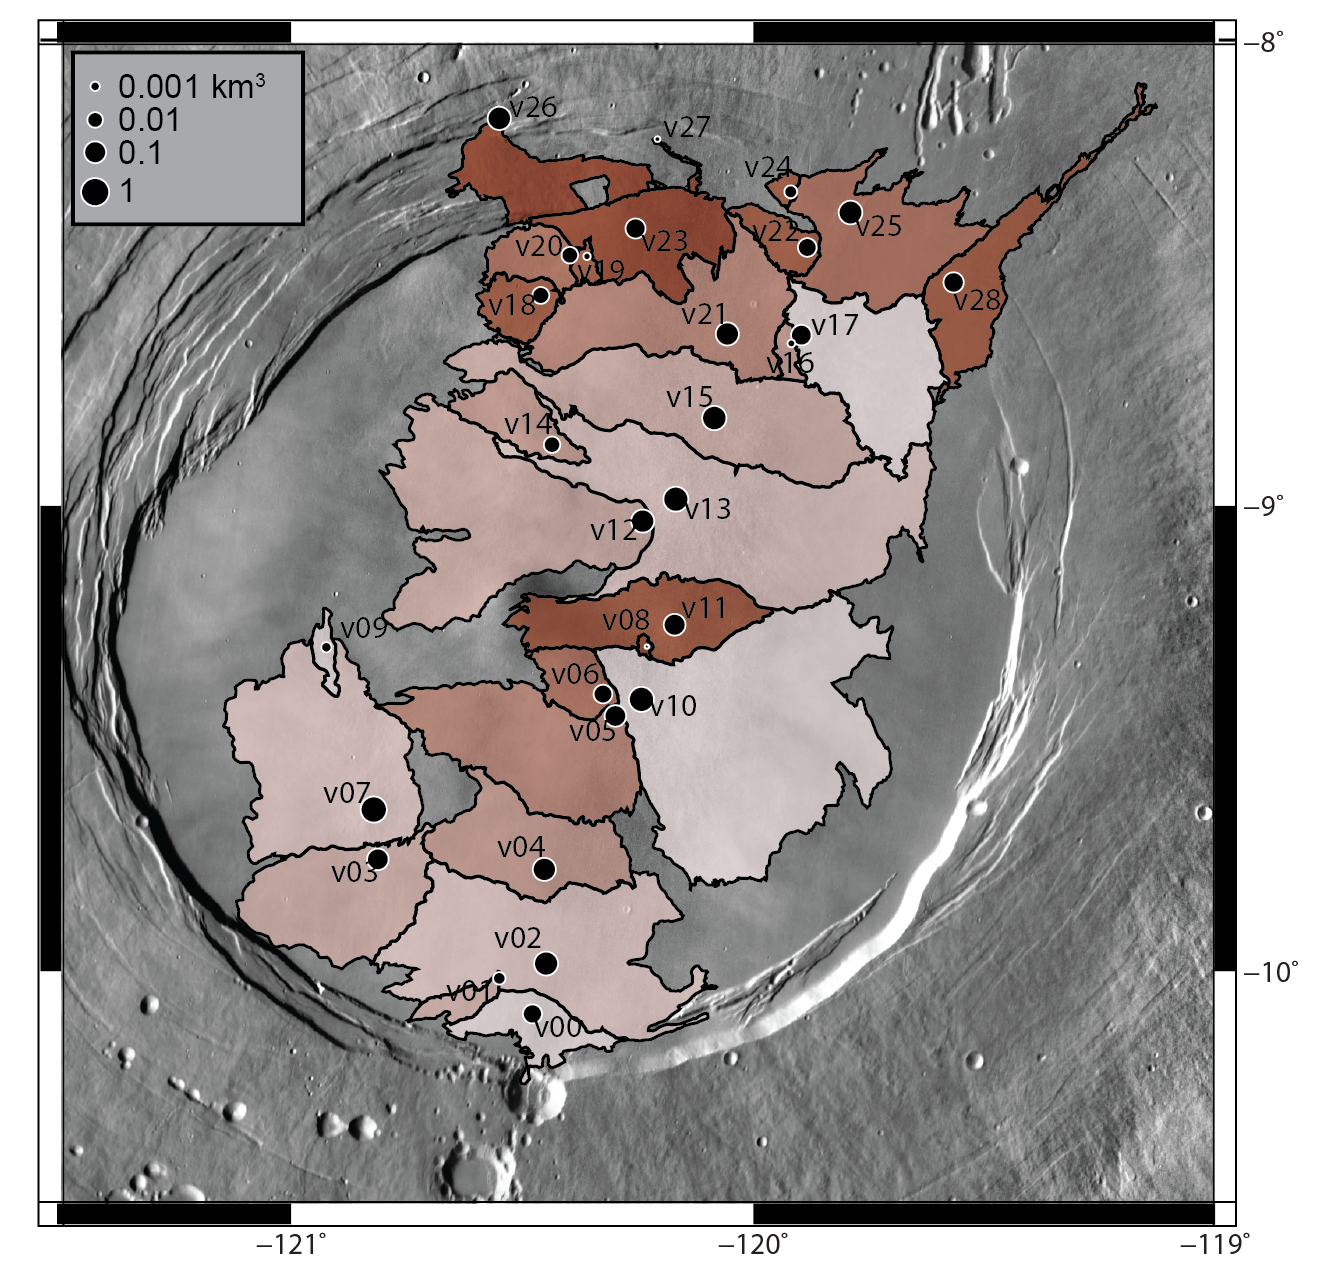
\includegraphics[width=0.5\textwidth]{figures/chapter-arsia/vent_map-01.png}
	}
	
	%Segue to VERRM
	\frame{\frametitle{Ages: Information Conflicts}
	%Examples: V00, V02, V04
	%          V25, V17
	}

	\frame{\frametitle{VERRM}
	%LPSC sketch
	}

\subsection{Results}
	\frame{\frametitle{Results}
	\centering
	\begin{block}{Recurrence Rate}
	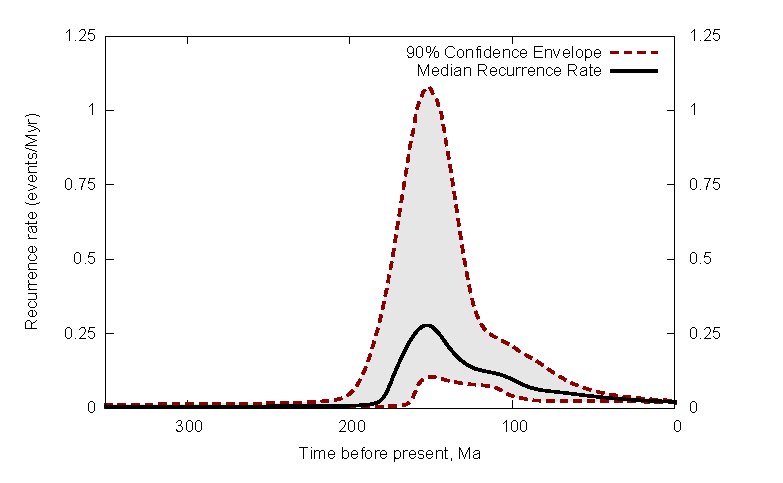
\includegraphics[width=0.6\textwidth]{figures/defense/VERRM_RR.eps}
	\end{block}
	}

	\frame{\frametitle{Volume Flux}
	\begin{columns}
	\column{0.5\textwidth}
	\centering
	\begin{block}{Sub-surface mesh model}
	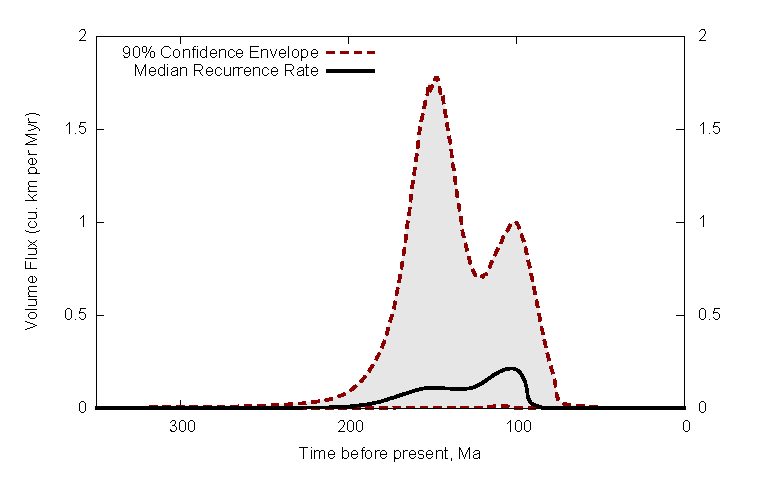
\includegraphics[width=1\textwidth]{figures/defense/VERRM_VF_MOLA.eps}
	\end{block}
	\column{0.5\textwidth}
	\centering
	\begin{block}{Thickness model}
	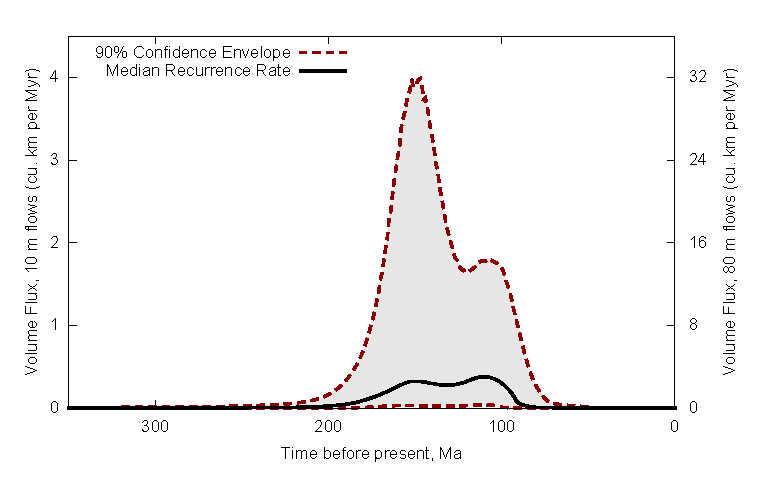
\includegraphics[width=1\textwidth]{figures/defense/VERRM_VF_THICK.eps}
	\end{block}
	\end{columns}
	}

\subsection{Implications}
	\frame{\frametitle{Tie in with Ashes and glaciers?}
	}

	\frame{\frametitle{Model of waning volcanism of Arsia}
	}

\section{Conclusions}
	\frame{\frametitle{Arsia Specific Conclusions}
	}

	\frame{\frametitle{Other Conclusions}
	}

\section{}
	\frame{\frametitle{Additional Thanks}
	}

	\frame{\frametitle{Questions?}
	}

\end{document}
